% GoldenGuide Software Design Document
% Build: pdflatex GoldenGuide-SDD.tex (run twice for the table of contents and cross-references)
\documentclass[11pt,letterpaper]{report}

% ---------------------------------------------------------------------------------------------
% Packages
% ---------------------------------------------------------------------------------------------
\usepackage[T1]{fontenc}
\usepackage[utf8]{inputenc}
\usepackage{lmodern}
\usepackage[margin=1in]{geometry}
\usepackage{microtype}
\usepackage{xcolor}
\usepackage{graphicx}
\usepackage{booktabs}
\usepackage{tabularx}
\usepackage{longtable}
\usepackage{array}
\usepackage{enumitem}
\usepackage{titlesec}
\usepackage{fancyhdr}
\usepackage{caption}
\usepackage{float}
\usepackage[most]{tcolorbox}
\usepackage{tikz}
\usetikzlibrary{positioning,arrows.meta,shapes.geometric,shapes.multipart,fit,backgrounds,calc}
\usepackage{url}
\usepackage[hidelinks]{hyperref}

% ---------------------------------------------------------------------------------------------
% Style
% ---------------------------------------------------------------------------------------------
\definecolor{lauPurple}{HTML}{330072}
\definecolor{lauGold}{HTML}{F2A900}
\definecolor{softPurple}{HTML}{EFEAF6}
\definecolor{softGold}{HTML}{FFF6DD}
\definecolor{softGrey}{HTML}{F4F4F4}
\definecolor{lineGrey}{HTML}{8A8A8A}

\hypersetup{colorlinks=true,linkcolor=lauPurple,urlcolor=lauPurple,citecolor=lauPurple}
\urlstyle{tt}
\DeclareUrlCommand\code{\urlstyle{tt}}
% Let long paths and identifiers wrap at separators.
\renewcommand{\UrlBreaks}{\do\/\do\-\do\_\do\.\do\<\do\>}

\titleformat{\chapter}[hang]{\Huge\bfseries\color{lauPurple}}{\thechapter}{0.6em}{}
\titlespacing*{\chapter}{0pt}{-10pt}{18pt}
\titleformat{\section}{\Large\bfseries\color{lauPurple}}{\thesection}{0.6em}{}
\titleformat{\subsection}{\large\bfseries}{\thesubsection}{0.6em}{}

\setlength{\parindent}{0pt}
\setlength{\parskip}{6pt}
\setlist{itemsep=2pt,topsep=4pt}
\renewcommand{\arraystretch}{1.25}
\newcolumntype{L}{>{\raggedright\arraybackslash}X}
\newcolumntype{P}[1]{>{\raggedright\arraybackslash}p{#1}}
\captionsetup{font=small,labelfont={bf,color=lauPurple}}

\pagestyle{fancy}
\fancyhf{}
\fancyhead[L]{\small\color{lineGrey}GoldenGuide --- Software Design Document}
\fancyhead[R]{\small\color{lineGrey}\leftmark}
\fancyfoot[C]{\small\thepage}
\renewcommand{\headrulewidth}{0.4pt}
\fancypagestyle{plain}{\fancyhf{}\fancyfoot[C]{\small\thepage}\renewcommand{\headrulewidth}{0pt}}

% Design decision record
\newtcolorbox{decision}[2]{enhanced,breakable,colback=softPurple,colframe=lauPurple,
  fonttitle=\bfseries,title={#1\quad #2},left=6pt,right=6pt,top=4pt,bottom=4pt,arc=2pt}
\newcommand{\field}[1]{\textbf{\color{lauPurple}#1:}~}
% Note box
\newtcolorbox{note}{colback=softGold,colframe=lauGold,left=6pt,right=6pt,top=3pt,bottom=3pt,arc=2pt}

% TikZ styles
\tikzset{
  every node/.append style={execute at begin node={\hyphenpenalty=10000\exhyphenpenalty=10000\relax}},
  box/.style={draw=lauPurple,fill=white,rounded corners=2pt,align=center,font=\footnotesize,
              minimum height=9mm,inner sep=4pt,text width=#1},
  box/.default=28mm,
  store/.style={cylinder,shape border rotate=90,aspect=0.18,draw=lauPurple,fill=softGold,
                align=center,font=\footnotesize,minimum height=12mm,text width=24mm,inner sep=2pt},
  ext/.style={draw=lineGrey,dashed,fill=softGrey,rounded corners=2pt,align=center,font=\footnotesize,
              minimum height=9mm,inner sep=4pt,text width=#1},
  ext/.default=28mm,
  arr/.style={-{Stealth[length=2.2mm]},thick,color=lauPurple!80!black},
  darr/.style={-{Stealth[length=2.2mm]},thick,dashed,color=lineGrey},
  lbl/.style={font=\scriptsize,fill=white,inner sep=1pt},
  group/.style={draw=lauPurple!50,fill=softPurple,rounded corners=4pt,inner sep=6pt},
  actor/.style={draw=lauPurple,fill=softPurple,rounded corners=2pt,font=\scriptsize\bfseries,
                minimum width=19mm,minimum height=7mm,align=center},
  msg/.style={-{Stealth[length=1.8mm]},thick,color=lauPurple!80!black},
  ret/.style={-{Stealth[length=1.8mm]},dashed,color=lineGrey},
  mlabel/.style={font=\scriptsize,above,inner sep=1pt,fill=white},
  snote/.style={draw=lauGold,fill=softGold,font=\scriptsize,align=center,inner sep=3pt},
}

% ---------------------------------------------------------------------------------------------
\begin{document}

% ---------------------------------------------------------------------------------------------
% Title page
% ---------------------------------------------------------------------------------------------
\begin{titlepage}
  \centering
  \vspace*{2cm}
  \IfFileExists{../../src/frontend/GoldenGuideLogo.png}{
\includegraphics[width=3cm]{../../src/frontend/GoldenGuideLogo.png}\par\vspace{1cm}}{}
  {\Huge\bfseries\color{lauPurple} GoldenGuide\par}
  \vspace{0.4cm}
  {\Large A grounded academic assistant for Wilfrid Laurier University\par}
  \vspace{1.5cm}
  {\color{lauGold}\rule{0.6\textwidth}{1.5pt}\par}
  \vspace{0.6cm}
  {\LARGE Software Design Document\par}
  \vspace{0.6cm}
  {\color{lauGold}\rule{0.6\textwidth}{1.5pt}\par}
  \vfill
  \begin{tabular}{@{}ll@{}}
    \textbf{Author} & Basleal Abshiro (b4sleal) \\
    \textbf{Version} & 1.2 \\
    \textbf{Date} & October 30, 2026 \\
    \textbf{Status} & Describes the implemented system \\
    \textbf{Repository} & \url{https://github.com/b4sleal/GoldenGuide} \\
    \textbf{Live system} & \url{https://askgoldenguide.ca} \\
  \end{tabular}
  \vspace{1.5cm}
\end{titlepage}

\pagenumbering{roman}
\chapter*{Revision History}
\addcontentsline{toc}{chapter}{Revision History}
\begin{tabularx}{\textwidth}{@{}lllL@{}}
\toprule
\textbf{Version} & \textbf{Date} & \textbf{Author} & \textbf{Changes} \\
\midrule
1.0 & 2026-10-30 & Basleal Abshiro & Initial release describing the implemented system: collection, storage, indexing, embedding service, question answering, security, configuration, observability, deployment and verification. \\
1.1 & 2026-10-30 & Basleal Abshiro & Added the staging environment and per-environment configuration files; corrected the description of retrieval profile fallback (semantic search only; no answer-model fallback configured). \\
1.2 & 2026-10-30 & Basleal Abshiro & Staging and production run their own Keycloak with a hosted realm that seeds the first administrator; each environment has its own Compose project name and data volumes; the pre-release database migrations were folded into a single baseline; the API documentation's inline script is allowed by hash in the content security policy. \\
\bottomrule
\end{tabularx}

\tableofcontents
\listoffigures
\listoftables

% =============================================================================================
\clearpage
\pagenumbering{arabic}
\chapter{Introduction}
% =============================================================================================

\section{Purpose}
This document describes the software design of GoldenGuide: what the system must do, how it is
structured to do it, and why each significant design choice was made. It is the reference for
anyone who maintains, extends, reviews or operates GoldenGuide. It follows the structure of IEEE 1016
(Software Design Descriptions): context, composition, logical, information, interface, interaction
and deployment viewpoints, with design rationale recorded alongside them.

\section{Problem statement}
Laurier students find academic information in several systems that do not talk to each other:
\begin{itemize}
  \item the \textbf{WLU websites} (policies, student services, deadlines, financial information);
  \item the \textbf{Academic Calendar} (courses, programs, requirements, regulations) for each academic year;
  \item \textbf{LORIS}, the registration system (term offerings: sections, CRNs, meeting times, seats, waitlists).
\end{itemize}
The existing Service Laurier assistant only answers pre-written questions. A question such as
\emph{``Can I take CP264 this winter, and when does it meet?''} requires the student to consult at
least two systems and understand how a calendar course relates to a term's sections.

\section{Goal}
A single conversational assistant that answers from all three official sources, cites every claim
with a working link, and states clearly when it cannot answer, built to production standards so it
can be operated, maintained and extended over the long term.

\section{Scope}
\begin{table}[H]
\centering
\caption{Scope}
\begin{tabularx}{\textwidth}{@{}LL@{}}
\toprule
\textbf{In scope} & \textbf{Out of scope} \\
\midrule
Answering questions from official WLU sources, with citations & Registering students or changing any WLU record \\
Collecting the Academic Calendar, WLU websites and LORIS on a schedule & Degree-planning advice beyond what sources state \\
Storing raw sources, structured records and vector indexes & Third-party ratings or community commentary as evidence \\
Administration: collection, indexing, job status, runtime settings, uploads & A replacement for LORIS or a full student portal \\
Sign-in with explicit roles, ready for WLU's identity provider & \\
\bottomrule
\end{tabularx}
\end{table}

\section{Intended audience}
Software engineers working on GoldenGuide; reviewers assessing its architecture; and technical readers interested in the design of
grounded retrieval-augmented generation (RAG) systems.

\section{Document overview}
Chapter~\ref{ch:requirements} lists requirements and constraints. Chapter~\ref{ch:architecture}
presents the architecture and Chapter~\ref{ch:decisions} the design decisions with their
alternatives. Chapters~\ref{ch:collection}--\ref{ch:cross} give the detailed design of each
subsystem, from crawling and storage to question answering. Chapters~\ref{ch:data}--\ref{ch:interaction}
cover data, interfaces and interactions. Chapters~\ref{ch:quality}--\ref{ch:risks} cover quality
attributes, deployment, verification, risks and the roadmap. Appendices contain a glossary, the
repository layout and the configuration catalogue.

% =============================================================================================
\chapter{Requirements and Constraints}\label{ch:requirements}
% =============================================================================================

\section{Functional requirements}
\begin{longtable}{@{}P{1.1cm}P{14.3cm}@{}}
\caption{Functional requirements}\label{tab:fr}\\
\toprule
\textbf{ID} & \textbf{Requirement} \\
\midrule
\endfirsthead
\toprule
\textbf{ID} & \textbf{Requirement} \\
\midrule
\endhead
F1 & Answer natural-language questions about courses, term offerings, prerequisites, registration, programs, policies, deadlines and services. \\
F2 & Answer factual lookups (prerequisites, sections, meeting times, rooms, instructors, seats) exactly as recorded in the source. \\
F3 & Cite the sources behind every answer with working links to the original pages. \\
F4 & Distinguish \emph{no records found}, \emph{operation unsupported}, \emph{a source failed} and \emph{results were limited} in the answer. \\
F5 & Resolve relative academic terms (``next term'', ``this fall'') to concrete terms from the current date, in code. \\
F6 & Stream answers progressively, ending with an explicit completion or failure signal. \\
F7 & Crawl the Academic Calendar and WLU websites, and download LORIS term offerings, storing raw sources. \\
F8 & Parse stored sources into structured records: courses, course terms (sections), programs and pages. \\
F9 & Index records for semantic search (chunk, enrich, embed) and re-index only what changed. \\
F10 & Run every collection and indexing step as an independently runnable, tracked, retryable job. \\
F11 & Refresh all sources nightly without manual intervention. \\
F12 & Let administrators run jobs, view their status, change runtime settings and upload documents. \\
F13 & Sign users in through an institutional OpenID Connect provider with explicitly mapped roles. \\
F14 & Let automation call administrative operations with narrowly scoped, revocable credentials. \\
\bottomrule
\end{longtable}

\section{Non-functional requirements}
\begin{longtable}{@{}P{1.1cm}P{3.0cm}P{11.2cm}@{}}
\caption{Non-functional requirements}\label{tab:nfr}\\
\toprule
\textbf{ID} & \textbf{Quality} & \textbf{Requirement} \\
\midrule
\endfirsthead
\toprule
\textbf{ID} & \textbf{Quality} & \textbf{Requirement} \\
\midrule
\endhead
N1 & Trustworthiness & Never fabricate courses, terms, prerequisites, policies or links; the answer model sees only retrieved evidence. \\
N2 & Provenance & Keep the source of every record; Academic Calendar and LORIS data never silently overwrite each other. \\
N3 & Reliability & One failing source degrades part of an answer, not all of it; failed ingestion work is retried without redoing successful work. \\
N4 & Security & Administrative operations require authorization; failures of sign-in or session state deny access; secrets never appear in code, YAML, images or logs. \\
N5 & Scalability & The API runs as multiple replicas without process-local shared state; services can run on separate machines. \\
N6 & Observability & Every request is traceable end to end through logs and traces by a single identifier. \\
N7 & Maintainability & Clear layer boundaries, typed configuration, provider replacement without changing use cases, behavioural tests. \\
N8 & Operability & One-command local setup with only Docker; bounded CPU and memory per service; reproducible builds. \\
N9 & Cost control & Use deterministic logic instead of an LLM where possible; bound prompt sizes; rate-limit public chat. \\
N10 & Politeness & Crawling respects \code{robots.txt}, uses conditional requests and bounded concurrency. \\
\bottomrule
\end{longtable}

\section{Constraints}
\begin{itemize}
  \item \textbf{Public sources only.} GoldenGuide reads public WLU pages and the public LORIS class
        search like a browser would. Their structure can change without notice.
  \item \textbf{No WLU system integration yet.} There is no data agreement with WLU; sign-in through
        WLU's Microsoft Entra ID tenant requires WLU to register the application.
  \item \textbf{External, paid, fallible LLMs.} Their output is untrusted input and their availability
        is not guaranteed.
  \item \textbf{Limited hardware.} Development and current production run on one PC with a consumer
        NVIDIA GPU; the system must also work CPU-only.
  \item \textbf{Parallel development.} Layer boundaries, ports and separately deployable services
        let several developers work on different parts (collection, retrieval, API, infrastructure)
        without stepping on each other; explicit structure and documentation are preferred over
        cleverness.
\end{itemize}

\section{Assumptions}
\begin{itemize}
  \item The Academic Calendar is published per academic year and is authoritative for course descriptions.
  \item LORIS is authoritative for term-specific sections and may differ from the calendar.
  \item Students accept answers that say part of a question could not be checked, provided they are told why.
\end{itemize}

% =============================================================================================
\chapter{Architecture}\label{ch:architecture}
% =============================================================================================

\section{Architectural style}
GoldenGuide is a \textbf{modular monolith}: one FastAPI backend containing the API and the
background jobs, plus a separate \textbf{embedding service}, with independently operated data stores.
Each runs in its own container with its own resource limits and Compose profile, so any of them can
be moved to another machine. Inside the backend, a \textbf{hexagonal (ports and adapters)}
architecture with domain-driven design keeps business logic independent of frameworks and vendors.

\section{System context}
\begin{figure}[H]
\centering
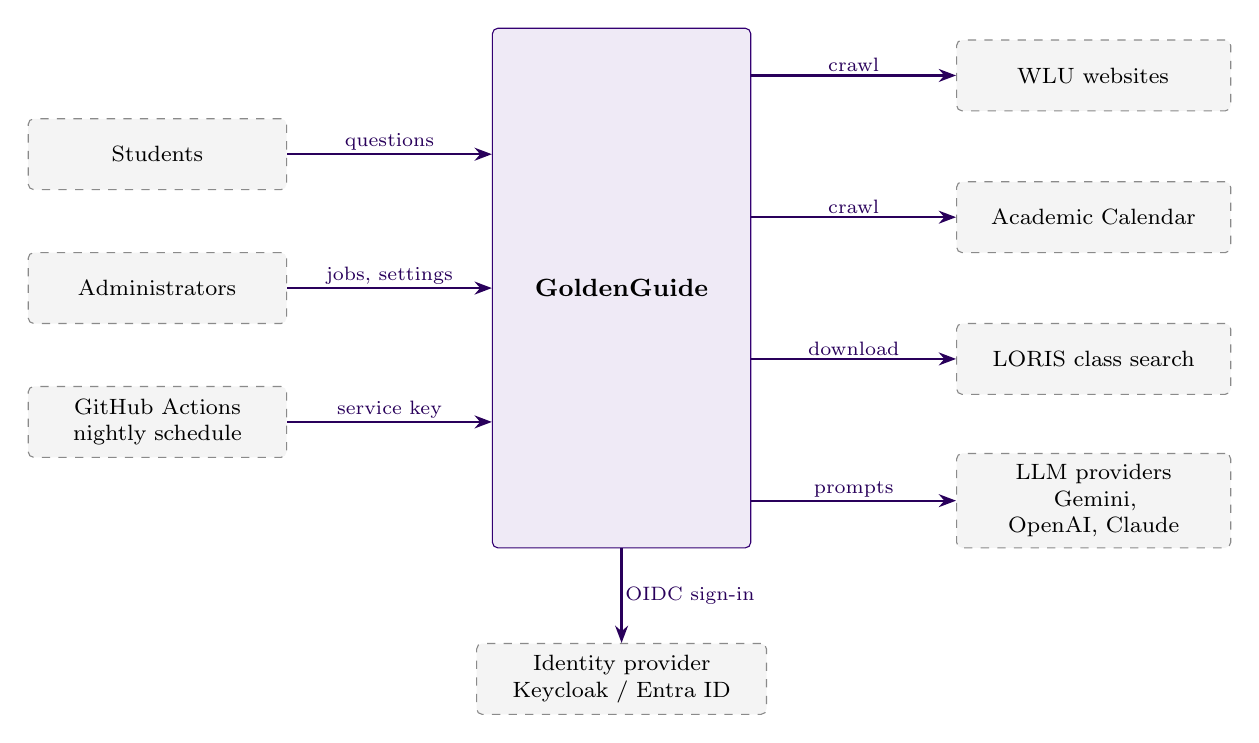
\begin{tikzpicture}[node distance=12mm and 26mm]
  \node[box=30mm,fill=softPurple,minimum height=66mm,font=\small\bfseries] (gg) {GoldenGuide};
  \node[ext=30mm,left=of gg,yshift=17mm] (st) {Students};
  \node[ext=30mm,left=of gg] (ad) {Administrators};
  \node[ext=30mm,left=of gg,yshift=-17mm] (gh) {GitHub Actions\\nightly schedule};
  \node[ext=32mm,right=of gg,yshift=27mm] (web) {WLU websites};
  \node[ext=32mm,right=of gg,yshift=9mm] (cal) {Academic Calendar};
  \node[ext=32mm,right=of gg,yshift=-9mm] (lor) {LORIS class search};
  \node[ext=32mm,right=of gg,yshift=-27mm] (llm) {LLM providers\\Gemini, OpenAI, Claude};
  \node[ext=34mm,below=12mm of gg] (idp) {Identity provider\\Keycloak / Entra ID};
  \draw[arr] (st.east) -- node[lbl,above]{questions} (gg.west |- st.east);
  \draw[arr] (ad) -- node[lbl,above]{jobs, settings} (gg);
  \draw[arr] (gh.east) -- node[lbl,above]{service key} (gg.west |- gh.east);
  \draw[arr] (gg.east |- web.west) -- node[lbl,above]{crawl} (web.west);
  \draw[arr] (gg.east |- cal.west) -- node[lbl,above]{crawl} (cal.west);
  \draw[arr] (gg.east |- lor.west) -- node[lbl,above]{download} (lor.west);
  \draw[arr] (gg.east |- llm.west) -- node[lbl,above]{prompts} (llm.west);
  \draw[arr] (gg) -- node[lbl,right]{OIDC sign-in} (idp);
\end{tikzpicture}
\caption{System context}\label{fig:context}
\end{figure}

\section{Container view}
\begin{figure}[H]
\centering
% Stores provision prepares sit in a column between provision (left) and backend (right),
% so provision's arrows run right and backend's run left without crossing.
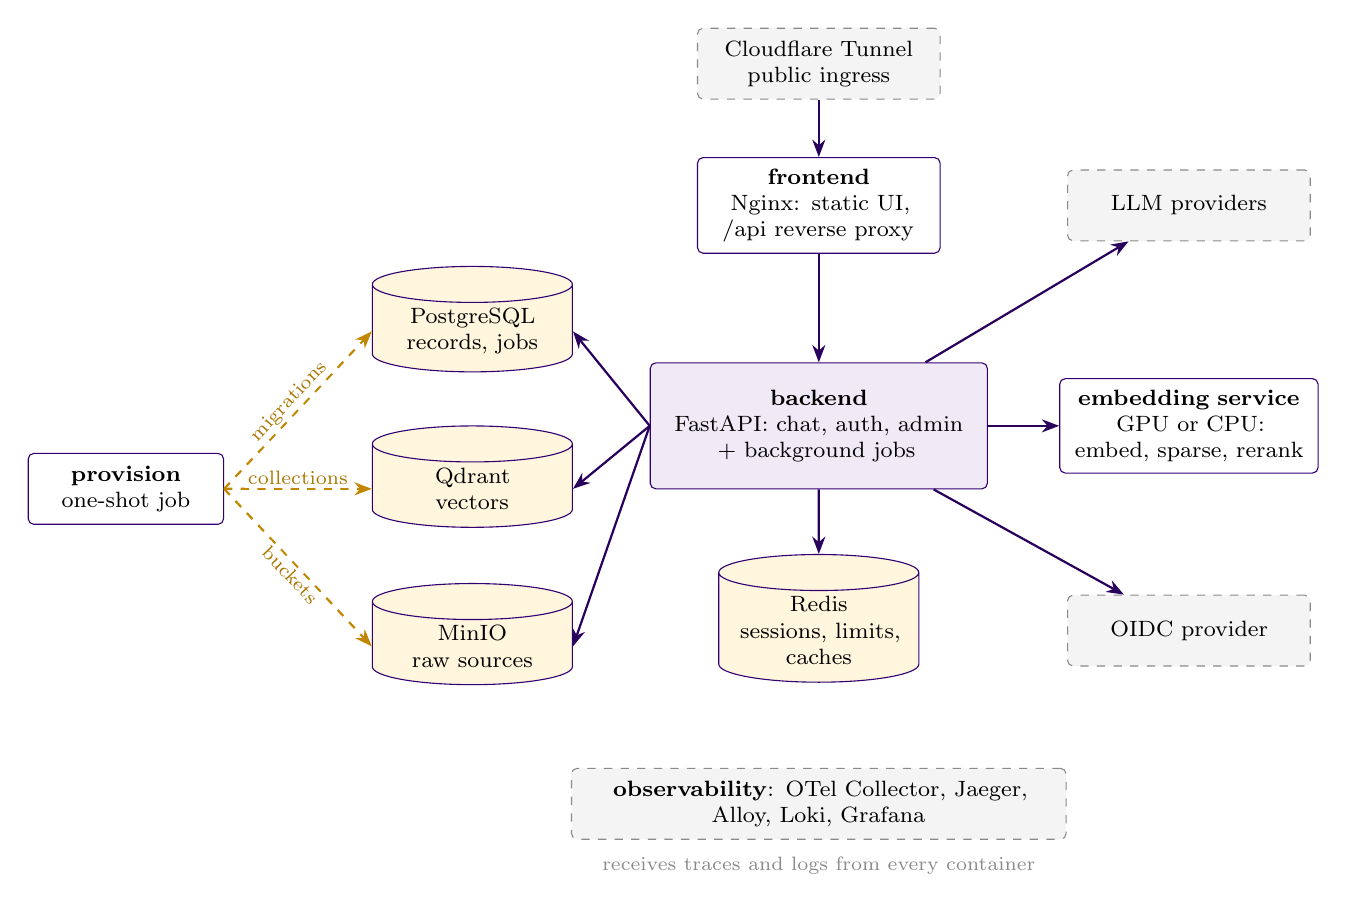
\begin{tikzpicture}
  \node[ext] (cf) at (1.2,6.4) {Cloudflare Tunnel\\public ingress};
  \node[box] (fe) at (1.2,4.6) {\textbf{frontend}\\Nginx: static UI,\\/api reverse proxy};
  \node[box=40mm,minimum height=16mm,fill=softPurple] (api) at (1.2,1.8) {\textbf{backend}\\FastAPI: chat, auth, admin\\+ background jobs};
  \node[store] (pg) at (-3.2,3.0) {PostgreSQL\\records, jobs};
  \node[store] (qd) at (-3.2,1.0) {Qdrant\\vectors};
  \node[store] (mn) at (-3.2,-1.0) {MinIO\\raw sources};
  \node[box=22mm] (prov) at (-7.6,1.0) {\textbf{provision}\\one-shot job};
  \node[store] (rd) at (1.2,-0.8) {Redis\\sessions, limits,\\caches};
  \node[box=30mm] (emb) at (5.9,1.8) {\textbf{embedding service}\\GPU or CPU:\\embed, sparse, rerank};
  \node[ext] (llm) at (5.9,4.6) {LLM providers};
  \node[ext] (idp) at (5.9,-0.8) {OIDC provider};
  \node[ext=60mm] (obs) at (1.2,-3.0) {\textbf{observability}: OTel Collector, Jaeger,\\Alloy, Loki, Grafana};
  \draw[arr] (cf) -- (fe);
  \draw[arr] (fe) -- (api);
  \draw[arr] (api) -- (emb);
  \draw[arr] (api) -- (llm);
  \draw[arr] (api) -- (idp);
  \draw[arr] (api) -- (rd);
  \foreach \s in {pg,qd,mn} \draw[arr] (api.west) -- (\s.east);
  \draw[arr,dashed,color=lauGold!80!black] (prov.east) -- node[lbl,above,sloped,text=lauGold!70!black]{migrations} (pg.west);
  \draw[arr,dashed,color=lauGold!80!black] (prov.east) -- node[lbl,above,text=lauGold!70!black]{collections} (qd.west);
  \draw[arr,dashed,color=lauGold!80!black] (prov.east) -- node[lbl,below,sloped,text=lauGold!70!black]{buckets} (mn.west);
  \node[font=\scriptsize,color=lineGrey,below=1mm of obs] {receives traces and logs from every container};
\end{tikzpicture}
\caption{Container view}\label{fig:containers}
\end{figure}

\begin{longtable}{@{}P{3.2cm}P{3.4cm}P{8.8cm}@{}}
\caption{Containers}\label{tab:containers}\\
\toprule
\textbf{Container} & \textbf{Built from} & \textbf{Responsibility} \\
\midrule
\endfirsthead
\toprule
\textbf{Container} & \textbf{Built from} & \textbf{Responsibility} \\
\midrule
\endhead
frontend & Nginx image & Serves the static UI and proxies \code{/api}, \code{/docs} and health routes to the backend, unbuffered for streaming. The browser only talks to this origin. \\
backend & Python runtime image (backend group) & FastAPI API (chat, sign-in, admin) and background jobs (crawling, parsing, indexing) as tracked tasks. \\
provision & Same image as backend & One-shot job before the API starts: Alembic migrations, MinIO buckets, Qdrant collections with version checks. Idempotent. \\
local-embedding-gpu / -cpu & Python runtime image (embedding group) & Separate service loading dense, sparse, multi-vector and reranking models; API-key protected. \\
postgres + db-bootstrap & postgres:16 & Authoritative structured data; the bootstrap job creates the databases. \\
qdrant & Locked version & Vector collections. \\
minio & Locked version & S3-compatible object storage for raw sources and uploads. \\
redis & redis:7-alpine & Critical session, OAuth and rate-limit state (append-only persistence) and optional caches. \\
keycloak & Keycloak 26 & OpenID Connect provider: a development realm locally, and a hosted realm (one Keycloak per environment) for staging and production. \\
observability & Upstream images & OpenTelemetry Collector, Jaeger, Alloy, Loki, Grafana. \\
tailscale, tunnel & Upstream images & Private network between machines; public ingress without inbound ports. \\
\bottomrule
\end{longtable}

\section{Logical view: backend layers}
\begin{figure}[H]
\centering
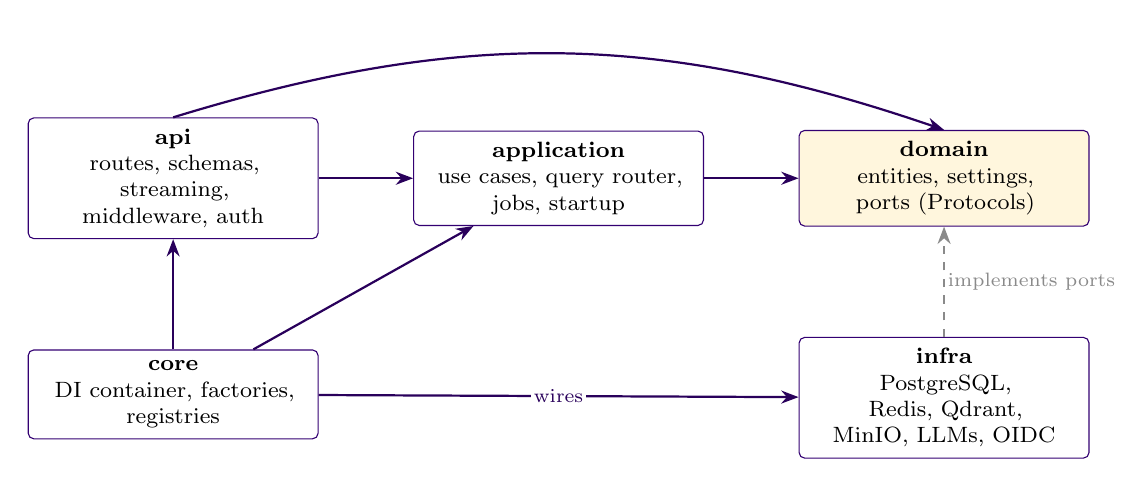
\begin{tikzpicture}[node distance=7mm and 12mm]
  \node[box=34mm] (apil) {\textbf{api}\\routes, schemas, streaming,\\middleware, auth};
  \node[box=34mm,right=of apil] (app) {\textbf{application}\\use cases, query router,\\jobs, startup};
  \node[box=34mm,right=of app,fill=softGold] (dom) {\textbf{domain}\\entities, settings,\\ports (Protocols)};
  \node[box=34mm,below=14mm of dom] (inf) {\textbf{infra}\\PostgreSQL, Redis, Qdrant,\\MinIO, LLMs, OIDC};
  \node[box=34mm,below=14mm of apil] (core) {\textbf{core}\\DI container, factories,\\registries};
  \draw[arr] (apil) -- (app);
  \draw[arr] (app) -- (dom);
  \draw[arr] (apil.north) to[bend left=18] (dom.north);
  \draw[darr] (inf) -- node[lbl,right]{implements ports} (dom);
  \draw[arr] (core) -- node[lbl]{wires} (inf);
  \draw[arr] (core) -- (app);
  \draw[arr] (core) -- (apil);
\end{tikzpicture}
\caption{Backend layers; arrows show allowed dependencies}\label{fig:layers}
\end{figure}

\begin{table}[H]
\centering
\caption{Layer responsibilities}\label{tab:layers}
\begin{tabularx}{\textwidth}{@{}P{2.4cm}P{4.6cm}L@{}}
\toprule
\textbf{Layer} & \textbf{Path} & \textbf{Owns} \\
\midrule
Domain & \code{src/backend/domain/} & Entities (\texttt{Course}, \texttt{CourseTerm}, academic terms, WLU pages, retrieval plans, evidence and outcomes, jobs, principals), typed settings, ports. No framework or vendor code. \\
Application & \code{src/backend/application/} & Use cases (chat, scraping, ingestion, settings), the query router, job runners, startup workflows. Depends only on domain ports. \\
Infrastructure & \code{src/backend/infra/} & Adapters: SQLAlchemy/asyncpg repositories and dialect operations, Redis stores, Qdrant, MinIO, LLM and embedding clients, text splitters, the OIDC client. \\
API & \code{src/backend/api/} & HTTP routes, request/response schemas, NDJSON streaming, middleware, authentication and authorization dependencies, rate limiting. \\
Composition root & \code{src/backend/core/} & Dependency-injection container, factories and provider registries; the provision job and service-key tool. \\
Shared & \code{src/goldenguide_common/} & Configuration loading, secret reading, structured logging and telemetry, shared by the backend and the embedding service. \\
\bottomrule
\end{tabularx}
\end{table}

% =============================================================================================
\chapter{Design Decisions}\label{ch:decisions}
% =============================================================================================
Each record states the decision, the alternatives considered, the rationale and the consequences.

\begin{decision}{D1}{Modular monolith rather than microservices}
\field{Decision} One backend codebase and process type. Separate containers only where the runtime
profile genuinely differs: the embedding service and the data stores.\par
\field{Alternatives} A service per capability (chat, ingestion, authentication).\par
\field{Rationale} One codebase, one release cadence and one domain model. Microservices would add network
failure modes, distributed transactions and deployment overhead with no scaling need behind them.
Hexagonal boundaries keep a later split possible.\par
\field{Consequences} Background jobs run inside the API process today (risk R1).
\end{decision}

\begin{decision}{D2}{Structured retrieval first; semantic search where it fits}
\field{Decision} Factual questions are compiled into typed SQL queries. Vector search handles policies,
services and open-ended questions. Both can contribute to one answer.\par
\field{Alternatives} ``Pure RAG'': embed everything and retrieve the top chunks for every question.\par
\field{Rationale} Chunk retrieval is probabilistic: it can miss the one section a student asked about,
confuse terms, or return 8 of 30 sections. Prerequisites and section times must be exact. SQL answers
exactly and cheaply; the LLM only chooses \emph{which} lookups to run.\par
\field{Consequences} More code (extraction, planning, compilation), justified by correctness on the most
common questions.
\end{decision}

\begin{decision}{D3}{Deterministic extraction before the LLM; validated plans}
\field{Decision} Course codes, subjects, rooms and instructors are recognised in code against the
database. The LLM plans only over masked entities, and its plan is validated before execution, with a
conservative fallback plan.\par
\field{Alternatives} Let the LLM read the raw question and emit queries or tool calls directly.\par
\field{Rationale} Code is exact and free. Masking means the LLM cannot invent a course. Validation means
a malformed or adversarial plan cannot trigger arbitrary queries.
\end{decision}

\begin{decision}{D4}{Hybrid vector search, cross-encoder reranking and whole-page expansion}
\field{Decision} Dense (MiniLM), sparse (SPLADE) and multi-vector (ColBERT) retrieval fused in Qdrant,
then a cross-encoder rerank, then whole pages when they fit the budget.\par
\field{Alternatives} Dense-only search; a hosted search service.\par
\field{Rationale} Dense vectors capture meaning but miss exact terms (``OSAP'', course codes); sparse
vectors catch terms; ColBERT adds token-level matching. A cross-encoder judges relevance rather than
similarity. Whole pages fix ``list everything'' questions that chunking fragments. A retrieval
evaluation measures each stage.\par
\field{Consequences} A GPU is preferred; every stage is optional per retrieval profile.
\end{decision}

\begin{decision}{D5}{A separate embedding service}
\field{Decision} Embedding, sparse vectorisation and reranking run in their own FastAPI service.\par
\field{Alternatives} Load models inside the backend; use only cloud embeddings.\par
\field{Rationale} PyTorch/CUDA images are several gigabytes and need a GPU; the API should stay small,
start fast and scale on CPU. The service can live on the one machine that has a GPU. Local models
avoid per-token costs during full re-indexes. CPU and GPU builds are mutually exclusive dependency
groups and can run side by side.
\end{decision}

\begin{decision}{D6}{Separated collection stages with raw sources kept}
\field{Decision} Discovery (crawling or downloading) stores raw HTML and LORIS extracts in object
storage and records each URL's outcome; parsing into records is a separate job; indexing is a
separate job again.\par
\field{Alternatives} Parse and embed while crawling, in one pass.\par
\field{Rationale} Each stage fails for different reasons (network, page structure, model). Keeping raw
sources means a parser fix is re-run without crawling WLU again; re-indexing never re-downloads.
Each stage reports its own outcome, so success of one is never reported as success of the pipeline.
\end{decision}

\begin{decision}{D7}{Ingestion as tracked, batched, idempotent jobs}
\field{Decision} Every collection and indexing step is a job with persisted run and batch state,
\texttt{fresh}/\texttt{update}/\texttt{retry} modes, heartbeats and a zombie sweep.\par
\field{Alternatives} A single ingestion script; a message queue and worker fleet.\par
\field{Rationale} Crawls and re-indexes are long and fail partially. Persisted batches let
\texttt{retry} replay exactly what failed; \texttt{update} processes only changed records. A durable
queue was deferred: it adds infrastructure without a current need, and the job ports allow a worker
later.\par
\field{Consequences} Endpoints answer \texttt{202 Accepted} with a status URL to poll.
\end{decision}

\begin{decision}{D8}{Configuration-driven providers and profiles}
\field{Decision} Providers, models, retrieval profiles, chunking, enrichment and prompts are layered
YAML, validated into typed settings and resolved through registries in the composition root.\par
\field{Alternatives} Constants in code; environment variables for everything.\par
\field{Rationale} Retrieval quality is tuned by experiment; changing a model or strategy should be a
reviewed configuration change. Typed validation fails at startup rather than mid-request.
Environment variables are reserved for deployment values and secrets.
\end{decision}

\begin{decision}{D9}{Redis for critical state with explicit failure policies}
\field{Decision} Sessions, single-use OAuth transactions and rate-limit windows live in Redis with
append-only persistence; caches live there too.\par
\field{Alternatives} Signed cookies (stateless sessions); in-process memory; PostgreSQL for sessions.\par
\field{Rationale} Server-side sessions are revocable and keep tokens out of the browser; shared state
lets every replica enforce the same limits.\par
\field{Consequences} Two opposite policies by design: critical state \textbf{fails closed}, caches
\textbf{fall back} to PostgreSQL.
\end{decision}

\begin{decision}{D10}{Provider-neutral OpenID Connect}
\field{Decision} Standard authorization-code flow with PKCE and nonce-verified ID tokens; everything
provider-specific comes from the discovery document; roles must be explicitly mapped.\par
\field{Alternatives} Keycloak-specific integration; custom username and password accounts.\par
\field{Rationale} WLU students and staff already have Microsoft accounts: moving from Keycloak to
Entra ID must be configuration. Explicit role mapping means a successful login never implies
privileges. No custom cryptography or session mechanisms.
\end{decision}

\begin{decision}{D11}{NDJSON streaming with an explicit terminal event}
\field{Decision} Answers stream as newline-delimited JSON events ending in \texttt{ok} or \texttt{error}.\par
\field{Alternatives} Server-Sent Events; WebSockets; one buffered response.\par
\field{Rationale} A plain streamed POST passes through every proxy and Cloudflare without upgrade
handling, carries typed events (text, citation, table, sources) and is trivial to parse. Once
streaming starts the HTTP status cannot change, so completion must be signalled in-band.
\end{decision}

\begin{decision}{D12}{Docker Compose with profiles as the deployment unit}
\field{Decision} One Compose definition with a profile per service group; development and production
overrides; one env file per environment (development, staging, production); CPU and memory limits on every container; loopback-bound ports; Tailscale between machines
and a Cloudflare Tunnel for public ingress.\par
\field{Alternatives} Kubernetes now; manual installation.\par
\field{Rationale} The only prerequisite for a contributor is Docker, and the same definition runs on
one PC or across machines. Kubernetes would be premature; the containers map directly to ECS or
Kubernetes later.
\end{decision}

% =============================================================================================
\chapter{Data Collection Subsystem}\label{ch:collection}
% =============================================================================================
This chapter covers how source data moves from WLU into GoldenGuide: discovery, raw storage and
parsing into structured records. Indexing for search is described in Chapter~\ref{ch:indexing}.

\section{Pipeline overview}
\begin{figure}[H]
\centering
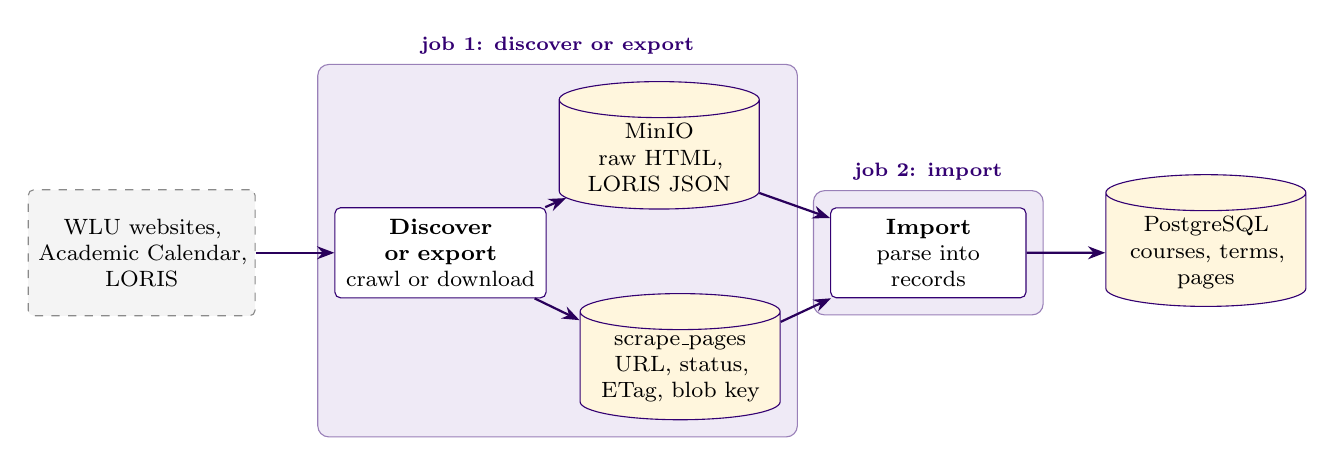
\begin{tikzpicture}[node distance=6mm and 8mm]
  \node[ext=26mm,minimum height=16mm] (src) {WLU websites,\\Academic Calendar,\\LORIS};
  \node[box=24mm,right=10mm of src] (disc) {\textbf{Discover}\\\textbf{or export}\\crawl or download};
  \node[store,above right=0mm and 8mm of disc] (blob) {MinIO\\raw HTML,\\LORIS JSON};
  \node[store,below right=0mm and 8mm of disc] (sp) {scrape\_pages\\URL, status,\\ETag, blob key};
  \node[box=22mm,right=36mm of disc] (imp) {\textbf{Import}\\parse into\\records};
  \node[store,right=10mm of imp] (db) {PostgreSQL\\courses, terms,\\pages};
  \begin{scope}[on background layer]
    \node[group,fit=(disc)(blob)(sp),label={[font=\scriptsize\bfseries,color=lauPurple]above:job 1: discover or export}] {};
    \node[group,fit=(imp),label={[font=\scriptsize\bfseries,color=lauPurple]above:job 2: import}] {};
  \end{scope}
  \draw[arr] (src) -- (disc);
  \draw[arr] (disc) -- (blob);
  \draw[arr] (disc) -- (sp);
  \draw[arr] (blob) -- (imp);
  \draw[arr] (sp) -- (imp);
  \draw[arr] (imp) -- (db);
\end{tikzpicture}
\caption{Collection: discovery and import are separate jobs}\label{fig:collection}
\end{figure}

\section{Sources}
\begin{table}[H]
\centering
\caption{Sources and their stages}\label{tab:sources}
\begin{tabularx}{\textwidth}{@{}P{2.6cm}LLP{3.0cm}@{}}
\toprule
\textbf{Source} & \textbf{Discover / export} & \textbf{Import} & \textbf{Stored as} \\
\midrule
Academic Calendar & Reads the calendar home page to find that year's calendars, seeds the crawl with every page of their search results, and crawls only that year's URLs. & Classifies each page (course, program, glossary, \ldots) and extracts the course header and details. & \code{courses}, \code{wlu_pages} \\
WLU websites (\texttt{wlu}, \texttt{students\_wlu}, \texttt{scholars\_wlu}) & Breadth-first crawl seeded from sitemaps and seed pages, restricted to each site's allowed domains and excluded paths. & Extracts title and main content (configured selector, noise removed). & \code{wlu_pages} \\
LORIS & Downloads one term's sections from the Banner class search into one JSON object. & Links each section to its calendar course and upserts it. & \code{course_terms} and children \\
\bottomrule
\end{tabularx}
\end{table}

\section{Crawler}
The crawler (\code{application/services/simple_scraping/}) is a breadth-first asynchronous crawler
built on \texttt{httpx}, driven by a \emph{site profile} that decides which URLs are seeds, which may be
followed and which are scraped.

\begin{itemize}
  \item \textbf{Gate.} Every URL requested --- seed, discovered link or redirect hop --- passes the same
        gate: the profile's rules (allowed domains, excluded path patterns, ignored file extensions
        such as PDFs and images) and \code{robots.txt}.
  \item \textbf{robots.txt} is parsed per RFC 9309: the group matching the crawler's user agent applies
        (else \texttt{*}), groups for the same agent are merged, the longest matching rule wins.
        An unavailable \code{robots.txt} is treated as disallowing the host (risk R4).
  \item \textbf{Conditional requests.} In \texttt{update} mode stored pages are re-checked with
        \texttt{If-None-Match} and \texttt{If-Modified-Since} headers built from the stored validators;
        \texttt{304 Not Modified} keeps the stored copy.
  \item \textbf{Change detection.} HTML is uploaded to object storage only when its content hash changed.
  \item \textbf{Bounded concurrency} (four concurrent requests in the nightly run) and structured progress
        logs (start, milestones, heartbeat, finish).
  \item \textbf{Errors.} A network failure on one page is stored as retryable and the crawl continues; a
        failure in processing or persistence aborts the crawl and marks the run failed.
\end{itemize}

\begin{table}[H]
\centering
\caption{Page statuses recorded in \texttt{scrape\_pages}}\label{tab:scrapestatus}
\begin{tabularx}{\textwidth}{@{}P{3.4cm}L@{}}
\toprule
\textbf{Status} & \textbf{Meaning} \\
\midrule
\texttt{pending} & Discovered, not yet fetched \\
\texttt{success} & Fetched HTML that the profile scrapes; stored in object storage \\
\texttt{skipped} & Fetched only to discover links (not scraped) \\
\texttt{empty} & Fetched, but no usable content \\
\texttt{retryable\_error} & Network failure; picked up by \texttt{retry} mode \\
\texttt{permanent\_error} & Non-200 or non-HTML response; not parsed \\
\bottomrule
\end{tabularx}
\end{table}

\begin{table}[H]
\centering
\caption{Crawl modes}\label{tab:crawlmodes}
\begin{tabularx}{\textwidth}{@{}P{2.2cm}L@{}}
\toprule
\textbf{Mode} & \textbf{Behaviour} \\
\midrule
\texttt{fresh} & Start from the profile's seeds and sitemaps; fetch everything (also finds new pages). \\
\texttt{update} & Re-check stored pages with conditional requests; only changed pages are stored again. \\
\texttt{retry} & Re-fetch pages that ended in a retryable error. \\
\bottomrule
\end{tabularx}
\end{table}

\section{Raw source storage}
Raw sources are kept in MinIO (S3-compatible) under deterministic keys, for example
\code{academic-calendar/2026-2027/courses/<sha256-of-url>.html}. Calendar pages are versioned by
academic year, so different years never collide. Each \code{scrape_pages} row records the URL, its
version, status, HTTP status, content type, blob key, content hash, ETag, Last-Modified, retry count and
timestamps (first seen, last attempted, last success), and a \code{needs_persistence} flag telling the
import job which pages changed.

\section{Parsing and import}
\begin{itemize}
  \item \textbf{Shared parsing} (\code{common_parsing.py}) converts HTML to clean Markdown using
        BeautifulSoup. Links in extracted text become numbered placeholders resolved when the text is
        shown, so stored text stays clean and links stay exact.
  \item \textbf{Academic Calendar import} parses a batch of stored pages and upserts them as courses or
        \code{wlu_pages} rows. Unknown subject codes \emph{block the batch} (they must be added to the
        WLU lexicon) rather than producing unmapped records. Pages that cannot be parsed are logged,
        skipped and stay flagged for the next run.
  \item \textbf{Website import} extracts the title (repeated site suffix removed) and the main content
        region, and upserts \code{wlu_pages} rows.
  \item \textbf{LORIS export.} Banner keeps search state in the session, so the client resets it, selects
        the term and pages through the results; each section's prerequisites, corequisites and
        restrictions are fetched and the whole term is stored as one JSON object.
  \item \textbf{LORIS import.} Unknown subject codes stop the import before anything is written. Courses
        missing from the calendar are inserted \emph{insert-only}, never overwriting calendar data. Each
        section is linked to its course for the governing academic year and upserted with its meetings
        and instructors. Sections whose course cannot be resolved are counted, not stored.
  \item \textbf{Audits.} Each crawl and import ends with an audit (page counts by status, record counts,
        a sample of unmapped pages) stored on the job run.
\end{itemize}

\begin{note}
\textbf{Provenance rule.} The Academic Calendar is authoritative for course descriptions; LORIS for
term sections. Credits and prerequisites can differ between them, so both are stored with their
source. Imports distinguish insert-only, upsert, fill-missing and conditional updates.
\end{note}

% =============================================================================================
\chapter{Job Runtime}\label{ch:jobs}
% =============================================================================================
All collection and indexing work runs through one job model (\code{application/services/jobs/}).

\begin{figure}[H]
\centering
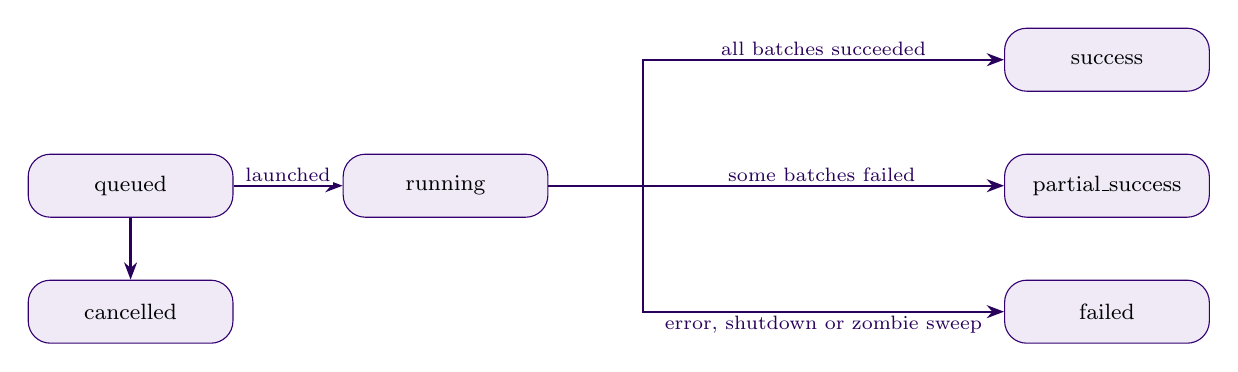
\begin{tikzpicture}[
  st/.style={draw=lauPurple,fill=softPurple,rounded corners=8pt,font=\footnotesize,minimum width=26mm,minimum height=8mm}]
  \node[st] (q) at (0,0) {queued};
  \node[st] (r) at (4,0) {running};
  \node[st] (s) at (12.4,1.6) {success};
  \node[st] (p) at (12.4,0) {partial\_success};
  \node[st] (f) at (12.4,-1.6) {failed};
  \node[st] (c) at (0,-1.6) {cancelled};
  \draw[arr] (q) -- node[lbl,above]{launched} (r);
  \draw[arr] (r.east) -- ++(1.2,0) |- node[lbl,above,pos=0.75]{all batches succeeded} (s.west);
  \draw[arr] (r.east) -- node[lbl,above,pos=0.6]{some batches failed} (p.west);
  \draw[arr] (r.east) -- ++(1.2,0) |- node[lbl,below,pos=0.75]{error, shutdown or zombie sweep} (f.west);
  \draw[arr] (q) -- (c);
\end{tikzpicture}
\caption{Job run lifecycle}\label{fig:joblifecycle}
\end{figure}

\begin{itemize}
  \item \textbf{Submission.} A run row is committed \texttt{queued}, the work is handed to the launcher,
        and the endpoint returns \texttt{202} with a status URL. Accepting a request is not completing it.
  \item \textbf{No overlap.} A second run of the same job name is refused (\texttt{409}) while one is
        queued or running, across all backend instances, using a PostgreSQL transaction advisory lock.
  \item \textbf{Batches.} Large jobs page through a table in id order (default 200 rows, up to three
        batches concurrently). A failed batch never aborts the others; it is stored \texttt{failed}
        with its error, and \texttt{retry} replays exactly those offsets.
  \item \textbf{Per-record failures.} One record failing does not stop its batch; the batch fails
        listing those records, which stay flagged for \texttt{retry} or \texttt{update}.
  \item \textbf{One-shot jobs} (a whole crawl, a LORIS export) use the same model with one synthetic
        batch, so every job shares one status and history view.
  \item \textbf{Heartbeats and recovery.} Running jobs send heartbeats. On shutdown, tasks are cancelled
        and awaited and interrupted runs recorded as failed. After a crash, a periodic zombie sweep
        (default: heartbeat older than five minutes, checked every two minutes) fails abandoned runs;
        their unfinished batches become retryable. Nothing is replayed automatically.
  \item \textbf{Scheduling.} A GitHub Actions workflow runs the full sequence nightly at 05:00
        America/Toronto with a scoped service key, waiting for each stage to succeed before the next.
\end{itemize}

% =============================================================================================
\chapter{Indexing Subsystem}\label{ch:indexing}
% =============================================================================================
Indexing turns structured records into searchable vectors. It reads PostgreSQL and writes Qdrant;
it never touches the original sources.

\begin{figure}[H]
\centering
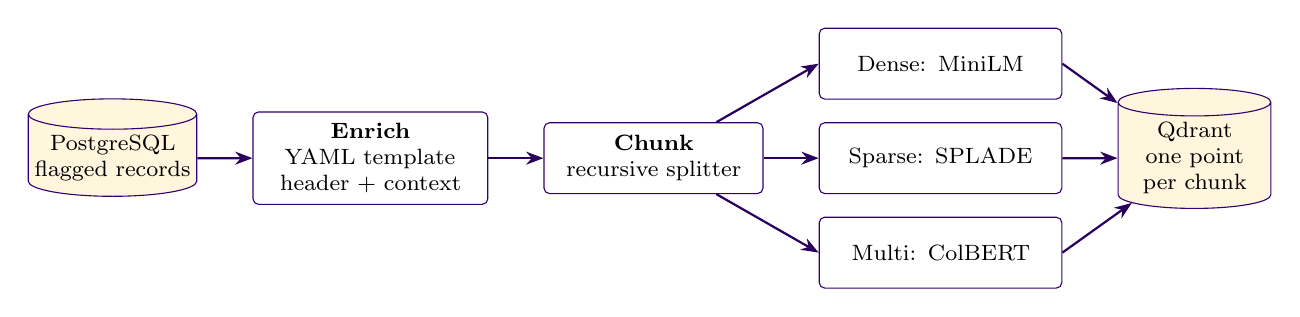
\begin{tikzpicture}[node distance=6mm and 7mm]
  \node[store,text width=20mm] (db) {PostgreSQL\\flagged records};
  \node[box=27mm,right=of db] (en) {\textbf{Enrich}\\YAML template\\header + context};
  \node[box=25mm,right=of en] (ch) {\textbf{Chunk}\\recursive splitter};
  \node[box=28mm,right=of ch,yshift=12mm] (d) {Dense: MiniLM};
  \node[box=28mm,right=of ch] (s) {Sparse: SPLADE};
  \node[box=28mm,right=of ch,yshift=-12mm] (m) {Multi: ColBERT};
  \node[store,right=of s,text width=18mm] (qd) {Qdrant\\one point\\per chunk};
  \draw[arr] (db) -- (en);
  \draw[arr] (en) -- (ch);
  \draw[arr] (ch) -- (d.west);
  \draw[arr] (ch) -- (s);
  \draw[arr] (ch) -- (m.west);
  \draw[arr] (d.east) -- (qd);
  \draw[arr] (s) -- (qd);
  \draw[arr] (m.east) -- (qd);
\end{tikzpicture}
\caption{Indexing: record to vectors}\label{fig:indexing}
\end{figure}

\section{Embedding job}
One embedding source per table (courses, course terms, WLU pages, uploaded documents) defines how to
page the table, build payloads and flag records. \texttt{fresh} embeds every record, \texttt{update}
only records whose \code{needs_embedding} flag is set (set on import when the content hash changed),
and \texttt{retry} re-runs the failed batches of the last run. The flag check happens in the job, not
in SQL, so a batch offset always covers the same rows and \texttt{retry} replays exactly what failed.

\section{Enrichment}
A chunk on its own often lacks context: ``Prerequisites: CP104'' does not say which course it belongs
to. Per record type (course, program, department, glossary, service page, \ldots) a template in
\code{configs/catalogs/text_enrichment/retrieval_text.yml} renders a header with identifying facts,
for example \emph{Academic Calendar Course: CP264 --- title; Subject; Academic Year; Prerequisites;
Credits}. Strategies (\texttt{minimal}, \texttt{deep}, \ldots) trade token overhead for context and are
chosen per vector collection.

\section{Chunking}
A recursive character splitter (LangChain) splits on paragraphs, then lines, then words. Presets range
from 300 to 1{,}500 characters with 200 characters of overlap and are chosen per collection; every
current collection uses the \texttt{large} preset (1{,}000 characters) with \texttt{deep} enrichment.

\section{Embedding and storage}
Each chunk is embedded with every vector type its collection defines and stored as one Qdrant point
with named vectors and a payload (source table, source id, URL, title, chunk text). A record's old
points are deleted \emph{only after} all new vectors were generated, so a failure keeps the previous
version searchable. Cloud embeddings (Gemini, OpenAI) are also supported per collection.

\begin{table}[H]
\centering
\caption{Vector collection layouts}\label{tab:collections}
\begin{tabularx}{\textwidth}{@{}P{2.6cm}L@{}}
\toprule
\textbf{Layout} & \textbf{Vectors} \\
\midrule
\texttt{dense} & Dense only \\
\texttt{sparse} & Dense + sparse (hybrid) \\
\texttt{multi} & Dense + ColBERT multi-vector \\
\texttt{multi\_sparse} & Dense + sparse + ColBERT multi-vector (current default) \\
\bottomrule
\end{tabularx}
\end{table}

Each collection carries a \emph{version}. Changing its chunking, enrichment or vectors requires a new
version and a re-index; provisioning refuses to run against an existing collection whose version does
not match, so incompatible vectors are never mixed.

% =============================================================================================
\chapter{Embedding Service}\label{ch:embedding}
% =============================================================================================
The embedding service (\code{src/embedding_service/}) is a separate FastAPI application that serves
every local model. It runs in one of two builds: \textbf{GPU} (CUDA PyTorch, ONNX Runtime GPU) or
\textbf{CPU} (CPU-only PyTorch wheels). The builds are mutually exclusive dependency groups but separate
containers can run side by side; the backend selects one with \code{EMBEDDING_RUNTIME} and the
service host and port.

\begin{table}[H]
\centering
\caption{Embedding service endpoints (all except health require an API key)}\label{tab:embapi}
\begin{tabularx}{\textwidth}{@{}P{4.2cm}L@{}}
\toprule
\textbf{Endpoint} & \textbf{Purpose} \\
\midrule
\texttt{GET /health} & Liveness (used by the container healthcheck) \\
\texttt{POST /embed/query} & Dense or multi-vector embedding of a question \\
\texttt{POST /embed/documents} & Dense or multi-vector embeddings of chunks (batched, at most 16 texts per request) \\
\texttt{POST /sparse/query}, \texttt{/sparse/documents} & SPLADE sparse vectors \\
\texttt{POST /rerank} & Cross-encoder scores for (question, passage) pairs \\
\bottomrule
\end{tabularx}
\end{table}

\begin{table}[H]
\centering
\caption{Local models}\label{tab:models}
\begin{tabularx}{\textwidth}{@{}P{2.6cm}P{4.4cm}LP{1.7cm}@{}}
\toprule
\textbf{Role} & \textbf{Model} & \textbf{Library} & \textbf{Runtime} \\
\midrule
Dense embedding & \code{all-MiniLM-L6-v2} & sentence-transformers & GPU, CPU \\
Multi-vector & \code{colbert-ir/colbertv2.0} & FastEmbed (late interaction) & GPU \\
Sparse vectors & \code{prithivida/Splade_PP_en_v1} & FastEmbed (sparse) & GPU \\
Reranker & \code{BAAI/bge-reranker-base} & sentence-transformers cross-encoder & GPU \\
Reranker & \code{cross-encoder/ms-marco-MiniLM-L-6-v2} & sentence-transformers cross-encoder & CPU \\
\bottomrule
\end{tabularx}
\end{table}

\begin{itemize}
  \item \textbf{Model loading.} The model registries are built when the service starts, and each
        model's constructor loads its weights, so every configured model for that runtime is
        downloaded into the \code{/models} volume (Hugging Face and FastEmbed caches) before requests
        are accepted. The healthcheck allows two minutes for the first start; later starts reuse the
        volume.
  \item \textbf{Registries.} Models are declared in \code{configs/catalogs/providers/ml\_local.yml} and
        mapped to implementations (MiniLM, FastEmbed ColBERT, SPLADE, cross-encoder) by a registry;
        adding a model type is one class and one registry entry.
  \item \textbf{Limits.} Thread counts are bounded (\code{EMBEDDING_THREADS}); the backend client uses a
        180-second timeout and batches documents.
  \item \textbf{Telemetry.} FastAPI instrumentation exports traces (health checks excluded); logs share the
        backend's JSON format.
\end{itemize}

% =============================================================================================
\chapter{Question Answering Subsystem}\label{ch:qa}
% =============================================================================================

\begin{figure}[H]
\centering
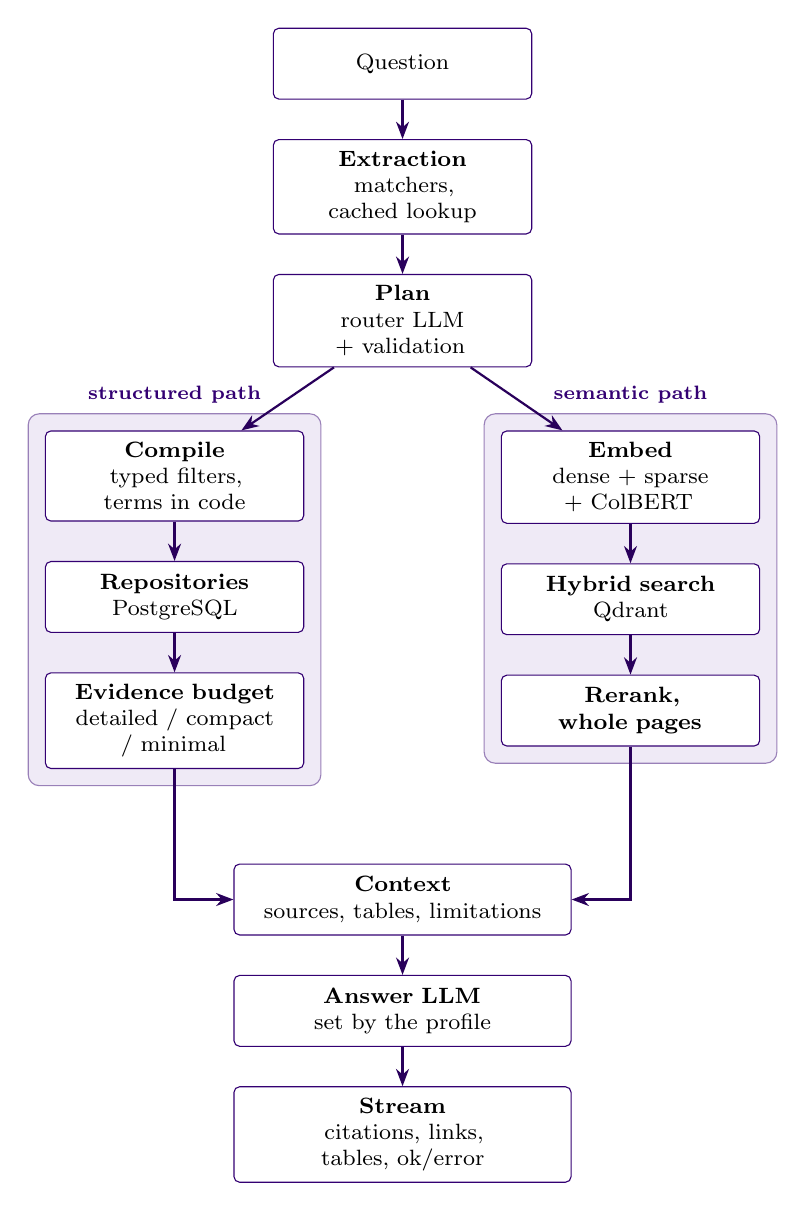
\begin{tikzpicture}[node distance=5mm and 6mm]
  \node[box=30mm] (q) {Question};
  \node[box=30mm,below=of q] (x) {\textbf{Extraction}\\matchers, cached lookup};
  \node[box=30mm,below=of x] (pl) {\textbf{Plan}\\router LLM + validation};
  \node[box=30mm,below left=8mm and -4mm of pl] (co) {\textbf{Compile}\\typed filters,\\terms in code};
  \node[box=30mm,below=of co] (re) {\textbf{Repositories}\\PostgreSQL};
  \node[box=30mm,below=of re] (bu) {\textbf{Evidence budget}\\detailed / compact / minimal};
  \node[box=30mm,below right=8mm and -4mm of pl] (em) {\textbf{Embed}\\dense + sparse + ColBERT};
  \node[box=30mm,below=of em] (hs) {\textbf{Hybrid search}\\Qdrant};
  \node[box=30mm,below=of hs] (rr) {\textbf{Rerank, whole pages}};
  \coordinate (mid) at (bu.south -| pl.south);
  \node[box=40mm,below=12mm of mid] (ctx) {\textbf{Context}\\sources, tables, limitations};
  \node[box=40mm,below=of ctx] (g) {\textbf{Answer LLM}\\set by the profile};
  \node[box=40mm,below=of g] (s) {\textbf{Stream}\\citations, links, tables, ok/error};
  \begin{scope}[on background layer]
    \node[group,fit=(co)(re)(bu),label={[font=\scriptsize\bfseries,color=lauPurple]above:structured path}] {};
    \node[group,fit=(em)(hs)(rr),label={[font=\scriptsize\bfseries,color=lauPurple]above:semantic path}] {};
  \end{scope}
  \draw[arr] (q) -- (x);
  \draw[arr] (x) -- (pl);
  \draw[arr] (pl) -- (co);
  \draw[arr] (pl) -- (em);
  \draw[arr] (co) -- (re);
  \draw[arr] (re) -- (bu);
  \draw[arr] (em) -- (hs);
  \draw[arr] (hs) -- (rr);
  \draw[arr] (bu) |- (ctx);
  \draw[arr] (rr) |- (ctx);
  \draw[arr] (ctx) -- (g);
  \draw[arr] (g) -- (s);
\end{tikzpicture}
\caption{Question answering pipeline}\label{fig:qa}
\end{figure}

\section{Retrieval profile}
A retrieval profile bundles the vector collection, search strategy, structured-evidence budget and
answer LLM, and may name fallback profiles that semantic search tries if it fails. Every question
currently uses \texttt{deep\_cloud} (\texttt{multi\_sparse} collection, hybrid + ColBERT search of 60
candidates, rerank to 20, whole pages up to 30{,}000 tokens). Its answer LLM is Gemini, and semantic
search falls back to \texttt{balanced\_cloud}. The settings also accept fallback answer models, but none
are configured.

\section{Deterministic entity extraction}
No LLM is used. Matchers check the question against an \emph{entity lookup} of every known course,
subject, program, room and instructor, built from the database and cached in Redis for a day (on a
cache outage the process uses its last copy or PostgreSQL). Recognised entities are masked
(\texttt{[COURSE1]}, \texttt{[DEPARTMENT1]}) before planning.

\begin{table}[H]
\centering
\caption{Entity matchers}\label{tab:matchers}
\begin{tabularx}{\textwidth}{@{}P{4.2cm}L@{}}
\toprule
\textbf{Matcher} & \textbf{Finds} \\
\midrule
Course code & \texttt{CP264}, \texttt{cp 264} and lexicon aliases (\texttt{comp sci 264}), kept only if the course exists \\
Lexicon & Faculties, departments and subjects by exact name or WLU alias (e.g.\ ``fhss'') \\
Department hint & Misspelled or truncated department names (fuzzy); passed to the planner, never masked \\
Room & LORIS room identifiers as students write them \\
Instructor & Full names of instructors teaching LORIS sections \\
\bottomrule
\end{tabularx}
\end{table}

\section{Query planning}
The router LLM turns the masked question into a retrieval plan: requests with a \emph{source}
(\texttt{courses}, \texttt{course\_terms}, \texttt{wlu\_pages}, \texttt{vector}), an \emph{operation}
(\texttt{lookup}, \texttt{filter}, \texttt{related}, \texttt{semantic}), entity masks and filters (term,
credit, level, days, rooms, instructors). LLM output enters the domain in one place and is:
\begin{enumerate}
  \item \textbf{leniently parsed}, repairing only shapes LLMs commonly get wrong (a single value where a
        list is expected), driven by the domain model's types;
  \item \textbf{validated}: each operation must be supported by its source and every mask must be one the
        extractor produced;
  \item \textbf{replaced by a fallback plan} if rejected: look up mentioned courses, otherwise semantic search.
\end{enumerate}

\section{Structured path}
\begin{enumerate}
  \item \textbf{Enrichment.} Every mentioned course receives a course lookup and a current-term offering
        lookup, even if the planner omitted one. Duplicate requests run once.
  \item \textbf{Compilation.} Course and course-term compilers turn each request into typed repository
        filters, one per (term, course or subject). Terms are resolved by the academic term resolver,
        never by the LLM. A filter the database cannot execute is reported as \emph{unsupported}.
  \item \textbf{Repositories} query PostgreSQL through domain ports, fetching one record beyond the limit
        to prove that more exist (``results limited'').
  \item \textbf{Evidence budget.} Each record has detailed, compact and minimal renderings; the whole set
        uses the richest tier the profile allows. If even the minimal tier does not fit, the request
        is reported as unsupported; records are never silently dropped.
  \item \textbf{Tables.} LORIS sections and planned listings become tables built from the exact records;
        the model places a table by writing \texttt{\{\{TABLE:n\}\}} instead of retyping rows.
\end{enumerate}

\section{Semantic path}
Runs when the plan requests it, or as a fallback when the structured path found nothing and the plan
allows it: embed the question with every vector type of the profile's collection, run hybrid search
in Qdrant, rerank with the cross-encoder, drop duplicate chunks, and replace chunks with whole pages
when the reranked pages fit the budget together. A failing provider moves to the next profile in the
profile's fallback list; if semantic search fails entirely, the answer is told so.

\section{Context assembly and generation}
\begin{itemize}
  \item Structured evidence first, then semantic results; each source is one numbered block with one
        citation entry.
  \item URLs are replaced by short placeholders that the model copies back and the stream restores, so
        the model never retypes or invents a link.
  \item Every request has an outcome --- completed (with count and truncation), unsupported or failed ---
        and the context tells the answer model which parts could not be answered and why.
  \item Today's date and the terms in scope are computed in code and given to the prompt.
  \item The answer is streamed through a chain applied to every chunk: citations
        (\texttt{[Source n]} $\rightarrow$ citation event) $\rightarrow$ links (placeholder $\rightarrow$ URL)
        $\rightarrow$ tables (marker $\rightarrow$ table event). Each stage holds back partial markers across
        chunk boundaries and releases them in order.
\end{itemize}

\begin{table}[H]
\centering
\caption{Retrieval outcomes and what the student sees}\label{tab:outcomes}
\begin{tabularx}{\textwidth}{@{}P{3.6cm}LL@{}}
\toprule
\textbf{Outcome} & \textbf{Meaning} & \textbf{Student sees} \\
\midrule
Completed, no records & The lookup ran and found nothing & ``No records found'' for that part \\
Unsupported & The plan asked for something not yet queryable & That part cannot be answered \\
Failed & A provider or the database failed & That part could not be checked right now \\
Truncated & Retrieval hit a limit & Results are partial; more exist \\
\bottomrule
\end{tabularx}
\end{table}

% =============================================================================================
\chapter{Cross-cutting Concerns}\label{ch:cross}
% =============================================================================================

\section{Authentication and authorization}
\begin{table}[H]
\centering
\caption{Access policy}\label{tab:access}
\begin{tabularx}{\textwidth}{@{}P{4.6cm}L@{}}
\toprule
\textbf{Caller} & \textbf{Can do} \\
\midrule
Anyone & Chat, rate-limited per client \\
Signed-in student & Same as anyone today; a student-only policy exists if WLU requires sign-in for chat. The student role is mapped only when the identity provider defines it; the bundled Keycloak realms define only the administrator role \\
Signed-in administrator & Every administrative route and the API documentation; holds every scope \\
Service client (bearer key) & Only its configured scopes: \texttt{sources:collect}, \texttt{indexing:sync}, \texttt{jobs:read}, \texttt{settings:write}, \texttt{documents:write} \\
This machine, sign-in disabled, \texttt{LOCAL\_ADMIN} on & Administrator, for development only; never through the tunnel, never in production \\
\bottomrule
\end{tabularx}
\end{table}

\begin{itemize}
  \item \textbf{Sign-in} uses the OpenID Connect authorization-code flow with PKCE (S256) and a nonce-bound
        ID token (Authlib, joserfc). The ID token's signature, issuer, audience, expiry and nonce are
        verified. Only explicitly configured roles count; a successful login alone grants nothing.
  \item \textbf{Sessions} are server-side in Redis; the browser holds only an opaque random cookie
        (\texttt{HttpOnly}, \texttt{SameSite=Lax}). Subjects are issuer-qualified.
  \item \textbf{Keycloak.} Development imports \code{deploy/keycloak/realm.json}, whose one user comes from
        \code{KC_TEST_ADMIN_USERNAME}, \code{KC_TEST_ADMIN_PASSWORD} and \code{KC_TEST_ADMIN_ROLE}. Staging and
        production each run their own Keycloak at their own HTTPS hostname (\code{KC_HOSTNAME}) with
        \code{deploy/keycloak/realm.hosted.json}: redirect URIs from \code{SITE_ORIGIN}, PKCE required,
        brute-force protection, no self-registration, and one seeded user, the first administrator
        (\code{KC_ADMIN_USERNAME}, \code{KC_ADMIN_PASSWORD}, \code{KC_ADMIN_ROLE}). The realm is imported
        only into an empty volume. The Keycloak console account (\code{KC_BOOTSTRAP_ADMIN_USERNAME}) is
        separate from GoldenGuide users. Keycloak still runs in its development mode (risk R13).
  \item \textbf{Microsoft Entra ID} is a configuration change (discovery URL, client, app roles), because
        no layer is Keycloak-specific.
  \item \textbf{Service keys} are stored only as SHA-256 hashes, two per client for rotation; a bearer
        request never falls back to the cookie.
  \item \textbf{Local administrator} (development): with sign-in disabled and \code{LOCAL_ADMIN} enabled,
        requests that did not pass through the Cloudflare tunnel (no \texttt{CF-Connecting-IP}) and come
        from a loopback or private peer are treated as an administrator. This relies on ports being bound
        to loopback; the backend refuses to start with it in production.
  \item \textbf{Fail closed.} No session store means no access; a missing credential stops production
        from starting; sign-in disabled without local admin returns \texttt{503}.
  \item \textbf{Hardening.} Same-origin checks on state-changing requests, a content security policy with
        configurable frame ancestors (the API documentation's inline initializer is allowed by its SHA-256 hash on
        that response only, never by allowing inline scripts), trusted hosts, an error boundary returning one envelope without
        internals, and per-client rate limits stored in Redis (forwarded addresses trusted only from
        configured proxies).
\end{itemize}

\section{Configuration}
Behaviour is versioned YAML; deployment values and secrets are environment variables.
\texttt{ConfigLoader} merges \code{configs/base/}, then \code{configs/catalogs/<group>/}, then
\code{configs/environments/<APP_ENV>.yml} (later wins), resolves references between entries and
\texttt{\$\{secrets:NAME\}} values through the \texttt{SecretReader} port, and validates the result into
typed Pydantic settings at startup. Catalogs follow one pattern:
\emph{providers} (things that exist), \emph{profiles} (reusable combinations), \emph{active}
(what this deployment uses). Some settings (prompts, model choices) can be changed at runtime by
administrators; they are versioned in PostgreSQL and cached in Redis. Appendix~\ref{app:config}
lists every configuration file.

\section{Observability}
\begin{itemize}
  \item \textbf{Logs.} Every service logs one JSON object per line (structlog) with \texttt{request\_id} and
        \texttt{trace\_id}; token-like fields are redacted. Alloy ships container logs to Loki with
        low-cardinality labels (service, container, level, host); \texttt{trace\_id} is structured metadata.
  \item \textbf{Traces.} OpenTelemetry instrumentation (FastAPI, httpx, SQLAlchemy, explicit spans) exports
        through the Collector to Jaeger.
  \item \textbf{Grafana} links each log line to its trace and each span to its logs.
  \item \textbf{Timings.} Each answer logs routing, structured, vector-search, first-chunk, generation and
        total times. Every error response carries \texttt{request\_id} and \texttt{trace\_id}.
\end{itemize}

% =============================================================================================
\chapter{Data Design}\label{ch:data}
% =============================================================================================

\section{Relational model}
\begin{figure}[H]
\centering
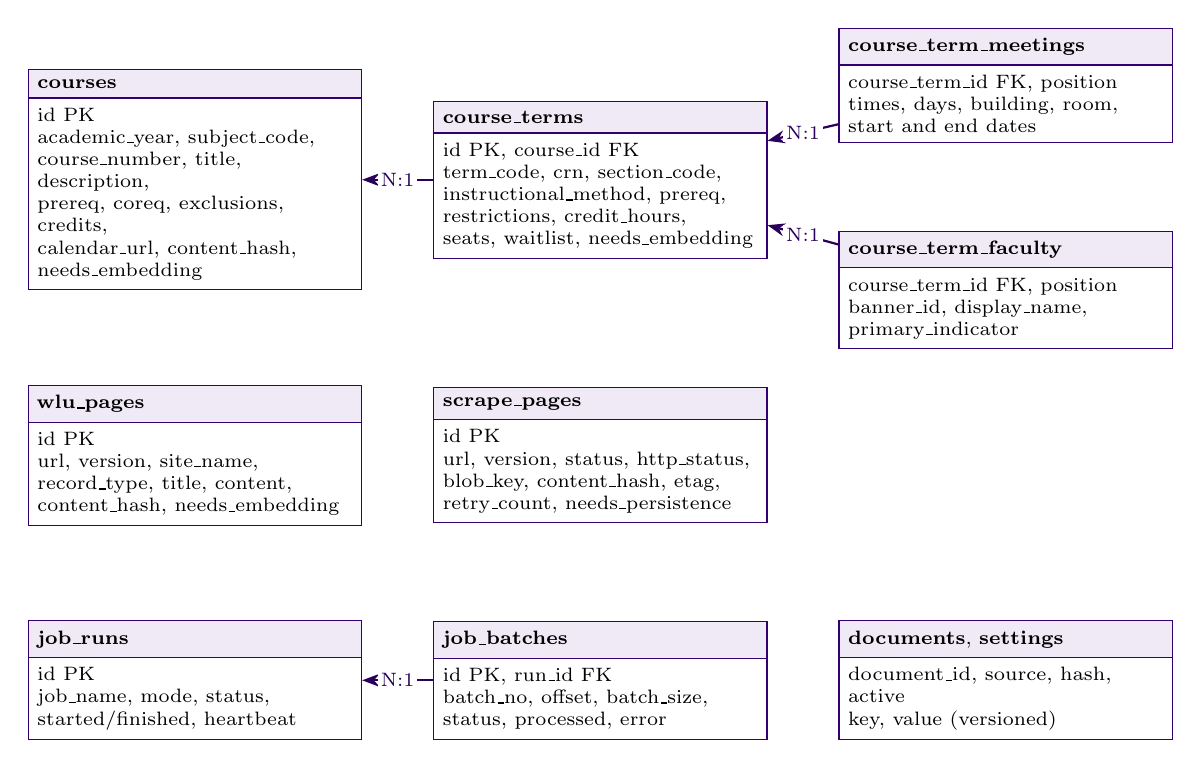
\begin{tikzpicture}[node distance=10mm and 9mm,
  ent/.style={rectangle split,rectangle split parts=2,draw=lauPurple,font=\scriptsize,
              text width=40mm,align=left,rectangle split part fill={softPurple,white}}]
  \node[ent] (courses) {\textbf{courses}\nodepart{two}id PK\\academic\_year, subject\_code,\\course\_number, title, description,\\prereq, coreq, exclusions, credits,\\calendar\_url, content\_hash,\\needs\_embedding};
  \node[ent,right=of courses] (terms) {\textbf{course\_terms}\nodepart{two}id PK, course\_id FK\\term\_code, crn, section\_code,\\instructional\_method, prereq,\\restrictions, credit\_hours,\\seats, waitlist, needs\_embedding};
  \node[ent,right=of terms,yshift=12mm] (meet) {\textbf{course\_term\_meetings}\nodepart{two}course\_term\_id FK, position\\times, days, building, room,\\start and end dates};
  \node[ent,right=of terms,yshift=-14mm] (fac) {\textbf{course\_term\_faculty}\nodepart{two}course\_term\_id FK, position\\banner\_id, display\_name,\\primary\_indicator};
  \node[ent,below=12mm of courses] (pages) {\textbf{wlu\_pages}\nodepart{two}id PK\\url, version, site\_name,\\record\_type, title, content,\\content\_hash, needs\_embedding};
  \node[ent,right=of pages] (scrape) {\textbf{scrape\_pages}\nodepart{two}id PK\\url, version, status, http\_status,\\blob\_key, content\_hash, etag,\\retry\_count, needs\_persistence};
  \node[ent,below=12mm of pages] (runs) {\textbf{job\_runs}\nodepart{two}id PK\\job\_name, mode, status,\\started/finished, heartbeat};
  \node[ent,right=of runs] (batches) {\textbf{job\_batches}\nodepart{two}id PK, run\_id FK\\batch\_no, offset, batch\_size,\\status, processed, error};
  \node[ent,right=of batches] (other) {\textbf{documents}, \textbf{settings}\nodepart{two}document\_id, source, hash, active\\key, value (versioned)};
  \draw[arr] (terms) -- node[lbl]{N:1} (courses);
  \draw[arr] (meet) -- node[lbl]{N:1} (terms);
  \draw[arr] (fac) -- node[lbl]{N:1} (terms);
  \draw[arr] (batches) -- node[lbl]{N:1} (runs);
\end{tikzpicture}
\caption{PostgreSQL entities (arrows point from child to parent)}\label{fig:er}
\end{figure}

\begin{table}[H]
\centering
\caption{Natural keys}\label{tab:keys}
\begin{tabularx}{\textwidth}{@{}P{3.6cm}P{5.6cm}L@{}}
\toprule
\textbf{Table} & \textbf{Unique key} & \textbf{Why} \\
\midrule
\texttt{courses} & academic year, institution, subject code, course number & A course is stable per calendar year (\texttt{Course} identity) \\
\texttt{course\_terms} & term code, CRN & A LORIS section is unique within its term (\texttt{CourseTerm} offering) \\
\texttt{wlu\_pages}, \texttt{scrape\_pages} & URL, version & The same page in different calendar years is a different record \\
\texttt{job\_batches} & run, batch number & A batch is replayed by position, never duplicated \\
\bottomrule
\end{tabularx}
\end{table}

\begin{itemize}
  \item \textbf{Course versus course term.} \texttt{courses} describes the calendar entry;
        \texttt{course\_terms} a term's sections, which can carry different credits, prerequisites and
        restrictions. Both keep their own copy with their source.
  \item \textbf{Change detection.} \texttt{content\_hash} detects real changes on import;
        \texttt{needs\_embedding} flags records for indexing and stays set when embedding fails.
  \item \textbf{Schema evolution} happens only through Alembic migrations applied by the provision job;
        the API refuses to serve an outdated schema; every migration must downgrade (tested). The
        pre-release migrations were folded into one baseline revision (\texttt{0001}); existing databases
        whose schema matched it were stamped to it without changing data.
\end{itemize}

\section{Vector, object and ephemeral data}
\begin{table}[H]
\centering
\caption{Non-relational stores}\label{tab:stores}
\begin{tabularx}{\textwidth}{@{}P{2.2cm}LP{4.2cm}@{}}
\toprule
\textbf{Store} & \textbf{Contents} & \textbf{Failure policy} \\
\midrule
Qdrant & One point per chunk: named vectors (dense, sparse, ColBERT) and payload (source, id, URL, title, text). Derived data, rebuildable from PostgreSQL; versioned collections. & Retrieval reports the semantic part as failed; the answer says so \\
MinIO & Raw calendar and website HTML (versioned keys), LORIS term extracts, uploaded originals. & Import jobs fail and are retried \\
Redis & Sessions; single-use OAuth transactions; rate-limit windows; caches for the entity lookup, settings and courses. & Critical state fails closed; caches fall back to PostgreSQL \\
\bottomrule
\end{tabularx}
\end{table}

% =============================================================================================
\chapter{Interface Design}\label{ch:interfaces}
% =============================================================================================

\section{HTTP API}
All routes are under \texttt{/api/v1}; administrators can browse OpenAPI documentation at \texttt{/docs}.

\begin{longtable}{@{}P{6.6cm}P{2.6cm}P{6.2cm}@{}}
\caption{HTTP endpoints}\label{tab:endpoints}\\
\toprule
\textbf{Method and path} & \textbf{Access} & \textbf{Purpose} \\
\midrule
\endfirsthead
\toprule
\textbf{Method and path} & \textbf{Access} & \textbf{Purpose} \\
\midrule
\endhead
\texttt{POST /chat/stream} & Public, rate-limited & Ask a question; NDJSON stream \\
\texttt{POST /chat/feedback} & Public & Planned (\texttt{501}) \\
\texttt{GET /auth/login}, \texttt{/auth/callback} & Public & OpenID Connect sign-in \\
\texttt{GET /auth/me}, \texttt{POST /auth/logout} & Signed in & Current principal; end session \\
\texttt{GET}, \texttt{PATCH /admin/settings/} & settings:write & Runtime defaults (versioned) \\
\texttt{GET} \code{/admin/documents/}, \texttt{POST} \code{.../upload} & documents:write & List and upload documents \\
\texttt{POST} \code{/admin/sources/academic-calendar/{discover,import}} & sources:collect & Calendar crawl; parse \\
\texttt{POST} \code{/admin/sources/websites/{discover,import}} & sources:collect & Website crawl; parse \\
\texttt{POST} \code{/admin/sources/registration/{export,import}} & sources:collect & LORIS download; load \\
\texttt{POST} \code{/admin/indexing/{courses,course-terms,pages}/sync} & indexing:sync & Build or update vectors \\
\texttt{GET /admin/jobs/\{run\_id\}} & jobs:read & Job status, batches, outcome \\
\texttt{GET /health/live} & Public & Liveness \\
\bottomrule
\end{longtable}

\section{Chat stream contract}
\begin{table}[H]
\centering
\caption{Stream events}\label{tab:events}
\begin{tabularx}{\textwidth}{@{}P{5.6cm}L@{}}
\toprule
\textbf{Event} & \textbf{Meaning} \\
\midrule
\texttt{\{"type": "text", "text": ...\}} & Answer text, in order \\
\texttt{\{"type": "citation", ...\}} & Citation marker with source numbers and URLs \\
\texttt{\{"type": "table", ...\}} & Table of database records, with title, columns and rows \\
\texttt{\{"type": "sources", ...\}} & Source list; always the last content event \\
\texttt{\{"type": "ok"\}} & Terminal: the answer is complete \\
\texttt{\{"type": "error", ...\}} & Terminal: failed after the stream started; same envelope as HTTP errors \\
\bottomrule
\end{tabularx}
\end{table}
An answer is complete only if the last event is \texttt{ok}; a stream ending without \texttt{ok} or
\texttt{error} is incomplete. Errors share one envelope: code, message, \texttt{request\_id},
\texttt{trace\_id}.

\section{Internal interfaces}
\begin{itemize}
  \item \textbf{Domain ports} (\code{src/backend/domain/ports/}): repositories, vector store, blob storage,
        caches and stores, LLM, embedding, reranker, sparse vectorizer, text splitter, job repository,
        secret reader. Adapters for vector stores and caches must pass shared contract test suites.
  \item \textbf{Embedding service API} (Table~\ref{tab:embapi}), protected by an API key.
  \item \textbf{Configuration} (Appendix~\ref{app:config}) and \textbf{telemetry} (OTLP, JSON logs).
\end{itemize}

% =============================================================================================
\chapter{Interaction Design}\label{ch:interaction}
% =============================================================================================

\section{Answering a question}
\begin{figure}[H]
\centering
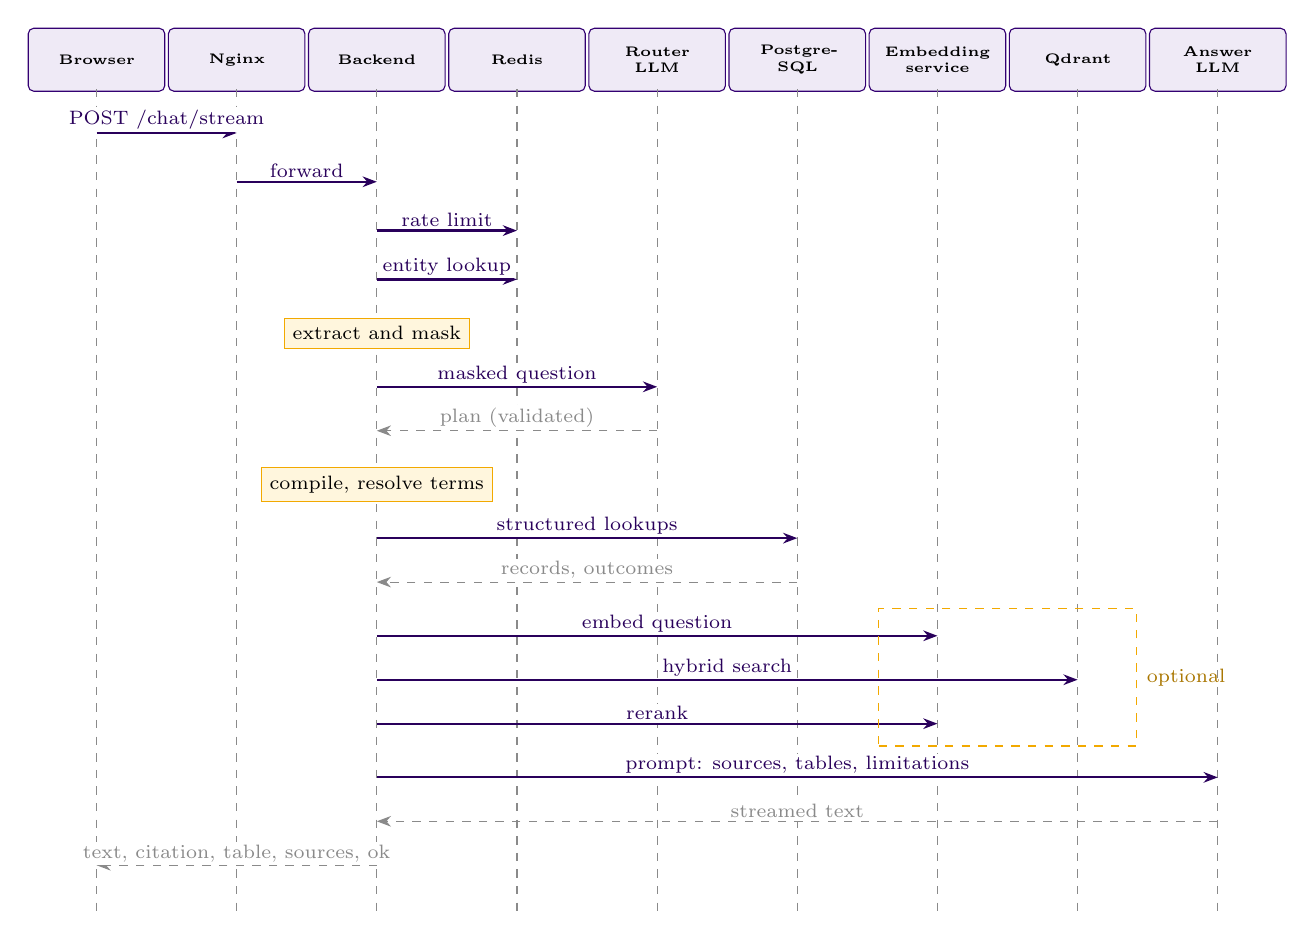
\begin{tikzpicture}[x=1.78cm,y=0.62cm]
  \foreach \x/\n in {0/Browser,1/Nginx,2/Backend,3/Redis,4/Router\\LLM,5/Postgre-\\SQL,6/Embedding\\service,7/Qdrant,8/Answer\\LLM}{
    \node[actor,minimum width=15mm,text width=15mm,font=\tiny\bfseries,minimum height=8mm] at (\x,0) {\n};
    \draw[dashed,color=lineGrey] (\x,-0.6) -- (\x,-17.5);
  }
  \draw[msg] (0,-1.5) -- node[mlabel]{POST /chat/stream} (1,-1.5);
  \draw[msg] (1,-2.5) -- node[mlabel]{forward} (2,-2.5);
  \draw[msg] (2,-3.5) -- node[mlabel]{rate limit} (3,-3.5);
  \draw[msg] (2,-4.5) -- node[mlabel]{entity lookup} (3,-4.5);
  \node[snote] at (2,-5.6) {extract and mask};
  \draw[msg] (2,-6.7) -- node[mlabel]{masked question} (4,-6.7);
  \draw[ret] (4,-7.6) -- node[mlabel]{plan (validated)} (2,-7.6);
  \node[snote] at (2,-8.7) {compile, resolve terms};
  \draw[msg] (2,-9.8) -- node[mlabel]{structured lookups} (5,-9.8);
  \draw[ret] (5,-10.7) -- node[mlabel]{records, outcomes} (2,-10.7);
  \draw[msg] (2,-11.8) -- node[mlabel]{embed question} (6,-11.8);
  \draw[msg] (2,-12.7) -- node[mlabel]{hybrid search} (7,-12.7);
  \draw[msg] (2,-13.6) -- node[mlabel]{rerank} (6,-13.6);
  \draw[msg] (2,-14.7) -- node[mlabel]{prompt: sources, tables, limitations} (8,-14.7);
  \draw[ret] (8,-15.6) -- node[mlabel]{streamed text} (2,-15.6);
  \draw[ret] (2,-16.5) -- node[mlabel]{text, citation, table, sources, ok} (0,-16.5);
  \node[font=\scriptsize,color=lineGrey,anchor=west] at (6.1,-12.7) {};
  \node[draw=lauGold,dashed,fit={(5.6,-11.3) (7.4,-14.0)},inner sep=1pt,
        label={[font=\scriptsize,color=lauGold!70!black]right:optional}] {};
\end{tikzpicture}
\caption{Sequence: answering a question}\label{fig:seqchat}
\end{figure}

\section{Signing in}
\begin{figure}[H]
\centering
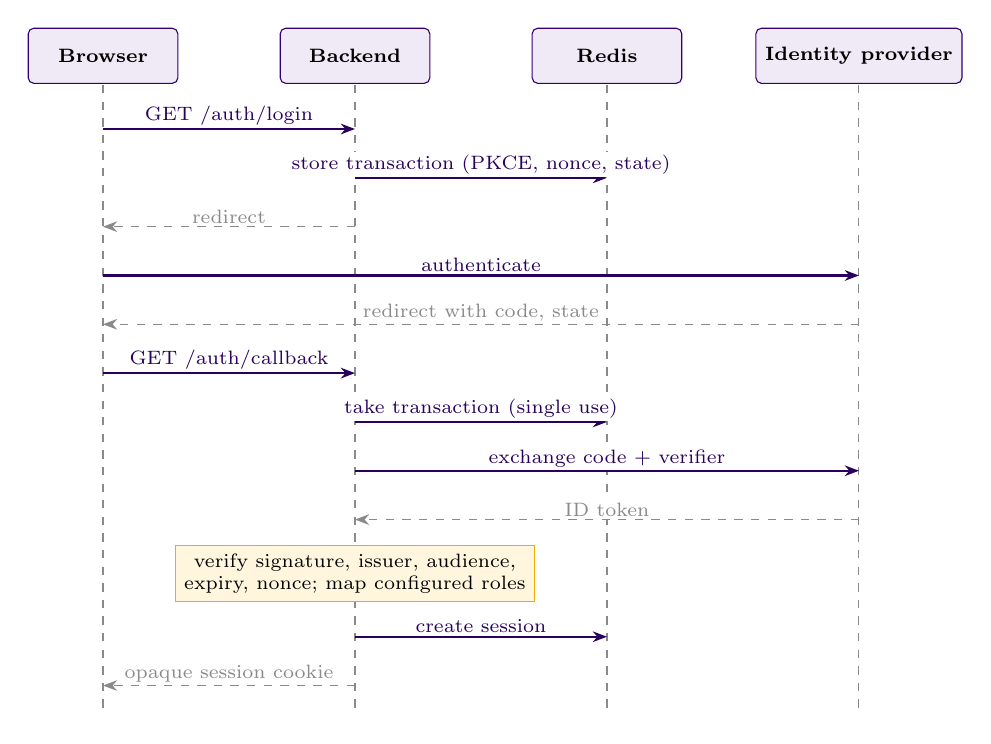
\begin{tikzpicture}[x=3.2cm,y=0.62cm]
  \foreach \x/\n in {0/Browser,1/Backend,2/Redis,3/Identity provider}{
    \node[actor] at (\x,0) {\n};
    \draw[dashed,color=lineGrey] (\x,-0.6) -- (\x,-13.5);
  }
  \draw[msg] (0,-1.5) -- node[mlabel]{GET /auth/login} (1,-1.5);
  \draw[msg] (1,-2.5) -- node[mlabel]{store transaction (PKCE, nonce, state)} (2,-2.5);
  \draw[ret] (1,-3.5) -- node[mlabel]{redirect} (0,-3.5);
  \draw[msg] (0,-4.5) -- node[mlabel]{authenticate} (3,-4.5);
  \draw[ret] (3,-5.5) -- node[mlabel]{redirect with code, state} (0,-5.5);
  \draw[msg] (0,-6.5) -- node[mlabel]{GET /auth/callback} (1,-6.5);
  \draw[msg] (1,-7.5) -- node[mlabel]{take transaction (single use)} (2,-7.5);
  \draw[msg] (1,-8.5) -- node[mlabel]{exchange code + verifier} (3,-8.5);
  \draw[ret] (3,-9.5) -- node[mlabel]{ID token} (1,-9.5);
  \node[snote] at (1,-10.6) {verify signature, issuer, audience,\\expiry, nonce; map configured roles};
  \draw[msg] (1,-11.9) -- node[mlabel]{create session} (2,-11.9);
  \draw[ret] (1,-12.9) -- node[mlabel]{opaque session cookie} (0,-12.9);
\end{tikzpicture}
\caption{Sequence: OpenID Connect sign-in}\label{fig:seqlogin}
\end{figure}

\section{Scheduled ingestion}
\begin{figure}[H]
\centering
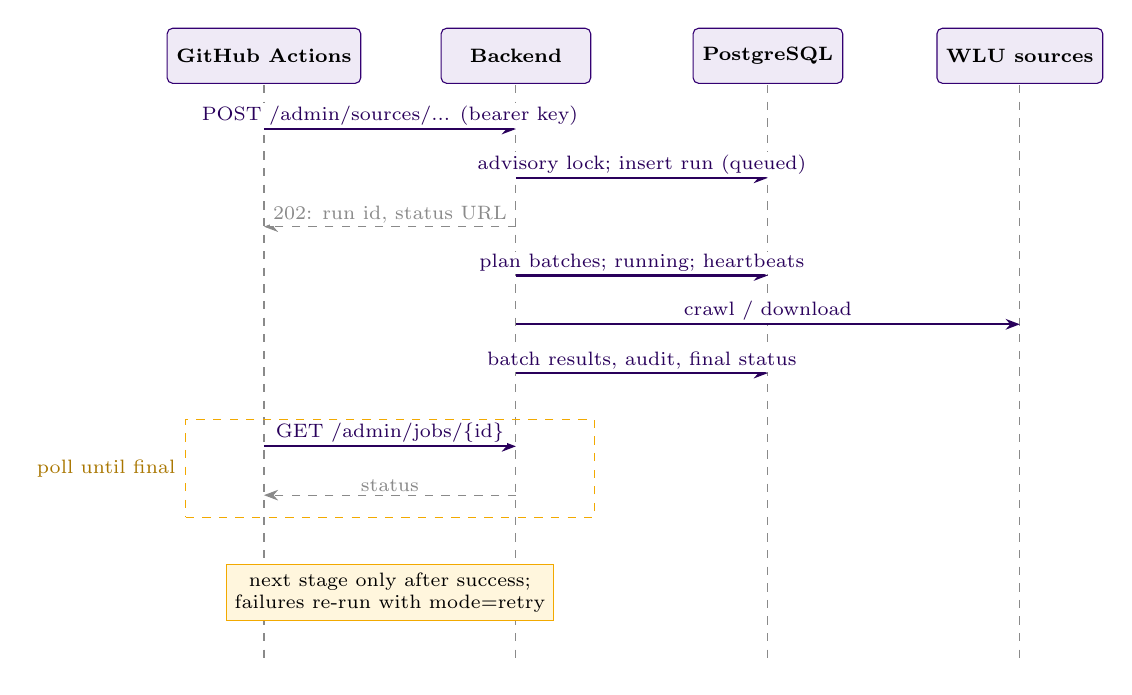
\begin{tikzpicture}[x=3.2cm,y=0.62cm]
  \foreach \x/\n in {0/GitHub Actions,1/Backend,2/PostgreSQL,3/WLU sources}{
    \node[actor] at (\x,0) {\n};
    \draw[dashed,color=lineGrey] (\x,-0.6) -- (\x,-12.5);
  }
  \draw[msg] (0,-1.5) -- node[mlabel]{POST /admin/sources/... (bearer key)} (1,-1.5);
  \draw[msg] (1,-2.5) -- node[mlabel]{advisory lock; insert run (queued)} (2,-2.5);
  \draw[ret] (1,-3.5) -- node[mlabel]{202: run id, status URL} (0,-3.5);
  \draw[msg] (1,-4.5) -- node[mlabel]{plan batches; running; heartbeats} (2,-4.5);
  \draw[msg] (1,-5.5) -- node[mlabel]{crawl / download} (3,-5.5);
  \draw[msg] (1,-6.5) -- node[mlabel]{batch results, audit, final status} (2,-6.5);
  \draw[msg] (0,-8.0) -- node[mlabel]{GET /admin/jobs/\{id\}} (1,-8.0);
  \draw[ret] (1,-9.0) -- node[mlabel]{status} (0,-9.0);
  \node[draw=lauGold,dashed,fit={(-0.3,-7.5) (1.3,-9.4)},inner sep=1pt,
        label={[font=\scriptsize,color=lauGold!70!black]left:poll until final}] {};
  \node[snote] at (0.5,-11.0) {next stage only after success;\\failures re-run with mode=retry};
\end{tikzpicture}
\caption{Sequence: a scheduled ingestion stage}\label{fig:seqjob}
\end{figure}

% =============================================================================================
\chapter{Quality Attributes}\label{ch:quality}
% =============================================================================================
\begin{longtable}{@{}P{3.2cm}P{12.2cm}@{}}
\caption{How each non-functional requirement is met}\label{tab:quality}\\
\toprule
\textbf{Requirement} & \textbf{Mechanisms} \\
\midrule
\endfirsthead
\toprule
\textbf{Requirement} & \textbf{Mechanisms} \\
\midrule
\endhead
N1 Trustworthiness & Evidence-only prompts; masked planning; validated plans; link placeholders; tables built from records; limitation notes \\
N2 Provenance & Separate course and course-term records; insert-only calendar protection; natural keys; raw sources kept; citations on every source \\
N3 Reliability & Per-request outcomes; profile fallback chains; batch-level retry; vectors replaced only after new ones exist; heartbeats and zombie sweep; separated collection stages \\
N4 Security & OIDC with PKCE and nonce; server-side sessions; explicit roles and scopes; hashed service keys; same-origin checks; security headers; fail-closed state; loopback-bound ports; required production secrets \\
N5 Scalability & Stateless API with shared Redis state; replica-safe job locks; per-service profiles; independently scaled embedding service \\
N6 Observability & JSON logs, OpenTelemetry traces, Grafana correlation, identifiers in every error, per-answer timings, job audits \\
N7 Maintainability & Hexagonal layers; dependency injection; registries; typed settings; behavioural unit tests and adapter contract tests \\
N8 Operability & Docker-only setup; working default environment; resource limits; locked image versions and lockfile; provision job \\
N9 Cost control & No LLM for extraction or term resolution; evidence token budgets; rate-limited chat; local embeddings; cheaper profiles available \\
N10 Politeness & RFC 9309 robots.txt handling; conditional requests; bounded concurrency; excluded paths and file types \\
\bottomrule
\end{longtable}

% =============================================================================================
\chapter{Deployment and Operations}\label{ch:deployment}
% =============================================================================================

\section{Environments}
\begin{table}[H]
\centering
\caption{Environments}\label{tab:envs}
\begin{tabularx}{\textwidth}{@{}P{3.0cm}L@{}}
\toprule
\textbf{Environment} & \textbf{Shape} \\
\midrule
Development & One machine, configured by \code{.env}: base Compose file plus development overrides (source mounts, auto-reload, shared development virtual environment, test database), Keycloak, full observability. A developer may expose it through their own Cloudflare Tunnel. \\
Staging & A production-style stack for the team (QA, staff), configured by \code{.env.staging}: the production Compose overrides with its own data stores, credentials, OIDC client and Cloudflare Tunnel at staging.askgoldenguide.ca, intended to be limited to the team by a Cloudflare Access policy. Today the backend's production-only startup checks (HTTPS origin, no \texttt{LOCAL\_ADMIN}, required trace exporter) apply only when \texttt{APP\_ENV} is \texttt{production} (risk R12). \\
Current production & Base Compose file plus production overrides (all credentials required), configured by \code{.env.prod}, on one self-hosted machine; public access through a Cloudflare Tunnel to askgoldenguide.ca; optional additional machines over Tailscale. \\
Planned cloud & ECS/Fargate for the API and provision job; a GPU instance for embeddings; RDS (PostgreSQL), ElastiCache (Redis), S3 (objects), managed or self-hosted Qdrant; Secrets Manager behind \texttt{SecretReader}; Entra ID for sign-in. \\
\bottomrule
\end{tabularx}
\end{table}

Each environment has its own env file, selected with \texttt{docker compose -{}-env-file}; the file also sets
\texttt{ENV\_FILE} so the containers read the same values. Only the \code{.env.dev.example},
\code{.env.staging.example} and \code{.env.prod.example} templates are committed. The staging and production
templates leave every credential blank, so a deployment cannot start with default passwords. In a larger
deployment the same values are injected as environment variables by a secret manager or the deployment
pipeline instead of a file. Each env file also sets \texttt{COMPOSE\_PROJECT\_NAME}
(\texttt{goldenguide-staging}, \texttt{goldenguide-prod}; development keeps \texttt{goldenguide}), so
containers, networks and volumes are separate per environment even on one machine. Staging and production
each expose their own Keycloak hostname (\texttt{auth-staging.askgoldenguide.ca}, \texttt{auth.askgoldenguide.ca})
through their tunnel; the administration console paths are limited to the team by a Cloudflare Access policy.

\section{Compose profiles and images}
Profiles select service groups (\texttt{database}, \texttt{vector-store}, \texttt{object-store},
\texttt{state\_store}, \texttt{provision}, \texttt{backend}, \texttt{frontend}, \texttt{auth},
\texttt{observability}, \texttt{log-shipper}, \texttt{tailnet}, \texttt{tunnel}); the aggregates
\texttt{all} includes everything except the embedding service, and \texttt{all-dev} also leaves out the
tunnel and Keycloak (sign-in is off in development; \texttt{auth} adds Keycloak). The embedding service is
chosen explicitly with \texttt{embedding-gpu} or \texttt{embedding-cpu} (or neither when another machine
runs it). One multi-stage Dockerfile builds every Python image: a non-root base, a toolchain with the
locked uv version, a development stage, a builder that installs one dependency group with
\texttt{uv sync -{}-locked}, and a minimal runtime stage without compilers.

\section{Resources and storage}
Every container has CPU and memory limits with swap disabled. Large dependencies are stored once:
runtime images carry each service's environment and are reused by development for the embedding
services; the development environment shares one volume between the uv cache and the virtual
environment so packages are hard-linked rather than copied. Model weights live in their own volumes.
Images that declare volumes receive a temporary file system so no anonymous volumes are created.
Qdrant and MinIO use locked image versions (pinned by digest: an exact image fingerprint rather than a
movable tag such as \texttt{latest}), so an update can never silently change how they store data on disk;
upgrading them is a deliberate step.

% =============================================================================================
\chapter{Verification}\label{ch:verification}
% =============================================================================================
\begin{table}[H]
\centering
\caption{Test strategy}\label{tab:tests}
\begin{tabularx}{\textwidth}{@{}P{2.4cm}P{4.2cm}L@{}}
\toprule
\textbf{Kind} & \textbf{Needs} & \textbf{Covers} \\
\midrule
Unit & Nothing (fakes at domain ports) & Extraction, term resolution, plan validation, compilers, evidence budgeting, streaming, authorization decisions, use cases \\
Integration & Real PostgreSQL, Redis, Qdrant & SQL filters and upserts, migrations (round trips), transactions, Redis atomicity and TTLs, Qdrant search; shared adapter contract suites \\
Evaluation & Running stack and data & Whether each benchmark question's answering page reaches the answer model, before and after reranking, with timings; end-to-end answers on demand \\
\bottomrule
\end{tabularx}
\end{table}

Integration tests use an isolated \texttt{goldenguide\_test} database (names must end in
\texttt{\_test}), a separate Redis database with random key prefixes and uniquely named Qdrant
collections, so development data is never touched. A missing test service skips locally and fails
in CI. GitHub Actions runs every unit and integration test on each pull request against disposable
service containers, without application secrets or paid LLM calls; a branch ruleset makes the check
mandatory.

% =============================================================================================
\chapter{Risks, Limitations and Roadmap}\label{ch:risks}
% =============================================================================================
\begin{longtable}{@{}P{0.9cm}P{5.0cm}P{3.6cm}P{5.9cm}@{}}
\caption{Risks and technical debt}\label{tab:risks}\\
\toprule
\textbf{ID} & \textbf{Item} & \textbf{Impact} & \textbf{Mitigation or plan} \\
\midrule
\endfirsthead
\toprule
\textbf{ID} & \textbf{Item} & \textbf{Impact} & \textbf{Mitigation or plan} \\
\midrule
\endhead
R1 & Jobs run inside the API process, not on a durable queue & A restart interrupts ingestion & Interrupted runs are recorded and retryable; a worker can implement the same job ports \\
R2 & WLU page structure can change & Parsers extract less & Audits record counts; nightly runs surface failures; raw HTML allows re-parsing \\
R3 & LLM outages or behaviour changes & Degraded answers & Plan validation; explicit error events; evaluation before changes. Retrieval profiles fall back on search failures; answer-model fallback is supported but not configured \\
R4 & An unavailable robots.txt disallows the host & A crawl can succeed with no pages & Logged; check audits, not only statuses \\
R5 & PostgreSQL and Redis connections are not encrypted & Exposure on untrusted networks & Keep them on loopback, private networks or Tailscale \\
R6 & Layer rules enforced by review, not tooling & Boundaries can erode & Add import-linter contracts to CI \\
R7 & Every question uses the deepest profile & Higher cost and latency & Route simple questions to cheaper profiles \\
R8 & No readiness endpoint & Orchestrators cannot detect broken dependencies & Add a dependency-aware readiness check \\
R9 & Questions and answers are logged & Student data in logs & Treat retention and access as student data \\
R10 & Chat is public & Abuse and cost & Redis-backed rate limits; student-only policy available \\
R11 & Local administrator relies on loopback-bound ports & Exposure if ports are published widely & Disabled by default; refused in production; documented \\
R12 & Staging does not enforce the production-only startup checks & Staging could run with an HTTP origin or \texttt{LOCAL\_ADMIN} that production would refuse & Apply the checks to staging as well; the staging template sets safe values \\
R13 & Staging and production Keycloak run in development mode with its built-in database & Limited durability and hardening of the identity provider & Suitable for a small team; move to production mode with PostgreSQL and backups, or to WLU's Entra ID \\
\bottomrule
\end{longtable}

\section{Roadmap}
\begin{enumerate}
  \item Microsoft Entra ID sign-in for students and faculty, with a faculty role.
  \item Course syllabi and faculty documents as sources.
  \item Routing simple questions to cheaper retrieval profiles.
  \item AWS deployment.
  \item Readiness endpoint, chat feedback and a durable job worker.
  \item Import-linter contracts and broader evaluation coverage in CI.
\end{enumerate}

% =============================================================================================
\appendix
% =============================================================================================
\chapter{Glossary}
\begin{longtable}{@{}P{4.0cm}P{11.4cm}@{}}
\toprule
\textbf{Term} & \textbf{Meaning} \\
\midrule
\endhead
Academic Calendar & WLU's official catalogue of courses, programs and regulations, per academic year \\
LORIS & WLU's registration system (Ellucian Banner); source of term offerings \\
CRN & Course Reference Number; identifies one section in one term \\
Course / CourseTerm & The stable calendar course versus one term's offering of it \\
RAG & Retrieval-augmented generation: answering with an LLM from retrieved evidence \\
Dense / sparse / multi-vector & Embedding styles: meaning (MiniLM), weighted terms (SPLADE), per-token vectors (ColBERT) \\
Cross-encoder & A model that scores a question and a passage together to reorder results \\
Retrieval profile & A named bundle of collection, search strategy, evidence budget and LLM, with optional fallback profiles for semantic search \\
Port / adapter & An interface defined by the domain / its implementation for a technology \\
Composition root & The one place where concrete adapters are chosen and wired \\
OIDC, PKCE & OpenID Connect sign-in; Proof Key for Code Exchange \\
Fail closed / fall back & On failure, deny (security state) / continue from another source (caches) \\
NDJSON & Newline-delimited JSON; one object per line \\
ETag & An HTTP validator used for conditional re-fetching \\
\bottomrule
\end{longtable}

\chapter{Repository Layout}
\begin{tabularx}{\textwidth}{@{}P{6.0cm}L@{}}
\toprule
\textbf{Path} & \textbf{Contents} \\
\midrule
\code{src/backend/} & FastAPI application (domain, application, infra, api, core, shared) \\
\code{src/embedding\_service/} & Embedding, sparse-vector and rerank service \\
\code{src/goldenguide_common/} & Code shared by backend and embedding service \\
\code{src/frontend/} & Static web interface \\
\code{configs/} & Layered YAML configuration (Appendix~\ref{app:config}) \\
\code{tests/backend/unit/}, \code{integration/} & Unit and integration tests mirroring the source layout \\
\code{tests/eval/} & Retrieval-quality evaluation \\
\code{docker/} & Our images: frontend, bootstrap script, development start script, BuildKit and daemon examples \\
\code{deploy/} & Configuration mounted into third-party services: Alloy, Loki, Grafana data sources, OpenTelemetry Collector, Keycloak realm \\
\code{scripts/} & Nightly ingestion client \\
\code{.github/workflows/} & Test gate and nightly ingestion \\
\code{docs/} & Documentation, including this document \\
\code{Dockerfile}, \code{docker-compose*.yml} & Images and the Compose stack \\
\code{.env.dev.example}, \code{.env.staging.example}, \code{.env.prod.example} & Environment variable templates; the populated files are not committed \\
\code{pyproject.toml}, \code{uv.lock} & Dependency groups and lockfile \\
\bottomrule
\end{tabularx}

\chapter{Configuration Catalogue}\label{app:config}
\begin{longtable}{@{}P{6.4cm}P{9.0cm}@{}}
\toprule
\textbf{File} & \textbf{Contents} \\
\midrule
\endhead
\code{base/system_config.yml} & Logging, OIDC client behaviour, job timing, service clients and scopes \\
\code{base/ai_behavior.yml} & Router and answer LLM prompts and defaults \\
\code{base/embedding_service.yml} & Embedding client: host, runtime, timeout, batch size \\
\code{catalogs/providers/infra.yml} & PostgreSQL, Redis, Qdrant and MinIO definitions \\
\code{catalogs/providers/ml_cloud.yml} & Cloud LLMs and embeddings \\
\code{catalogs/providers/ml_local.yml} & Local embedding, sparse and reranking models per runtime \\
\code{catalogs/providers/text_splitter.yml} & Chunk sizes and overlaps \\
\code{catalogs/profiles/vector_collection.yml} & Collection layouts and versions \\
\code{catalogs/profiles/vector_retrieval.yml} & Search depth, reranking and whole-page budgets \\
\code{catalogs/profiles/db_evidence.yml} & Structured-evidence token budgets per tier \\
\code{catalogs/profiles/retrieval_profile.yml} & Retrieval profiles with their fallback profiles \\
\code{catalogs/active/infra.yml} & Stores in use for each role \\
\code{catalogs/router/router.yml} & Entity lookup cache settings \\
\code{catalogs/scraping/websites.yml} & Websites: sitemaps, seeds, domains, selectors, exclusions \\
\code{catalogs/text_enrichment/retrieval_text.yml} & Enrichment templates per record type \\
\code{catalogs/text_enrichment/wlu_lexicon.yml} & Faculties, departments, subjects and aliases \\
\code{catalogs/institution/institution.yml} & Institution code, time zone, registration URL \\
\code{environments/<APP_ENV>.yml} & Development, staging and production overrides \\
\bottomrule
\end{longtable}

\end{document}
